\documentclass[11pt,3p,review,authoryear]{elsarticle}

%\documentclass{document}

% use packages
% \usepackage{ecrc} %required for elsarticle https://www.elsevier.com/researcher/author/policies-and-guidelines/latex-instructions
\usepackage[utf8]{inputenc}
\usepackage{amsmath}
\usepackage{amsthm}
\usepackage{amsfonts}
\usepackage{amscd}
\usepackage{amssymb}
\usepackage{natbib}
\usepackage{url}
\usepackage[table,xcdraw,usenames]{xcolor}
%\usepackage[usenames]{color}

\usepackage{graphicx}
\usepackage{subcaption}
\usepackage{mathtools}
\usepackage{enumitem}
\usepackage{bm}
\usepackage{comment}
\usepackage{pdfpages}

\usepackage{hyperref}
\usepackage{caption}
\usepackage{float}
%\usepackage[caption = false]{subfig}
\usepackage{tikz}
\usepackage{multirow}
\usepackage[linesnumbered, ruled,vlined]{algorithm2e}
\usepackage{pdflscape}
\usepackage{etoolbox}

%\AtBeginEnvironment{align}{\setcounter{equation}{0}} % https://tex.stackexchange.com/questions/349247/how-do-i-reset-the-counter-in-align

% margin setup
\usepackage{geometry}
\geometry{margin=0.8in}

% function definition
\newcommand{\weight}{\pi}
\newcommand{\ret}{\textbf{r}}
\newcommand{\y}{\textbf{y}}
\newcommand{\w}{\textbf{w}}
\newcommand{\x}{\textbf{v}}
\newcommand{\dbf}{\textbf{d}}
\newcommand{\X}{\textbf{X}}
\newcommand{\Y}{\textbf{Y}}
\newcommand{\V}{\textbf{V}}
%\newcommand{\L}{\textbf{L}}
\newcommand{\Hist}{\mathcal{H}}
\newcommand{\Prob}{\mathbb{P}}
\def\mbf#1{\mathbf{#1}} % bold but not italic
\def\ind#1{\mathrm{1}(#1)} % indicator function
\newcommand{\simiid}{\stackrel{iid}{\sim}} %[] IID 
\def\where{\text{ where }} % where
\newcommand{\indep}{\perp \!\!\! \perp } % independent symbols
\def\cov#1#2{\mathrm{Cov}(#1, #2)} % covariance 
\def\mrm#1{\mathrm{#1}} % remove math
\newcommand{\reals}{\mathbb{R}} % Real number symbol
\def\t#1{\tilde{#1}} % tilde
\def\normal#1#2{\mathcal{N}(#1,#2)} % normal
\def\mbi#1{\boldsymbol{#1}} % Bold and italic (math bold italic)
\def\v#1{\mbi{#1}} % Vector notation
\def\mc#1{\mathcal{#1}} % mathical
\DeclareMathOperator*{\argmax}{arg\,max} % arg max
\DeclareMathOperator*{\argmin}{arg\,min} % arg min
\def\E{\mathbb{E}} % Expectation symbol
\def\mc#1{\mathcal{#1}}
\def\var#1{\mathrm{Var}(#1)} % Variance symbol
\def\checkmark{\tikz\fill[scale=0.4](0,.35) -- (.25,0) -- (1,.7) -- (.25,.15) -- cycle;} % checkmark
\newcommand\red[1]{{\color{red}#1}}
\def\bs#1{\boldsymbol{#1}}
\def\P{\mathbb{P}}
\def\var{\mathbf{Var}}
\def\naturals{\mathbb{N}}
\def\cp{\overset{p}{\to}}
\def\clt{\overset{\mathcal{L}^2}{\to}}

\setcounter{tocdepth}{4}
\setcounter{secnumdepth}{4}

\newtheorem{corollary}{Corollary}
\newcommand{\ceil}[1]{\lceil #1 \rceil}
\newcommand{\norm}[1]{\left\lVert#1\right\rVert} % A norm with 1 argument
\DeclareMathOperator{\Var}{Var} % Variance symbol

\newtheorem{cor}{Corollary}
\newtheorem{lem}{Lemma}
\newtheorem{thm}{Theorem}
\newtheorem{defn}{Definition}
\newtheorem{prop}{Proposition}
\theoremstyle{definition}
\newtheorem{remark}{Remark}
\hypersetup{
  linkcolor  = blue,
  citecolor  = blue,
  urlcolor   = blue,
  colorlinks = true,
} % color setup

% proof to proposition 
\newenvironment{proof-of-proposition}[1][{}]{\noindent{\bf
    Proof of Proposition {#1}}
  \hspace*{.5em}}{\qed\bigskip\\}
% general proof of corollary
  \newenvironment{proof-of-corollary}[1][{}]{\noindent{\bf
    Proof of Corollary {#1}}
  \hspace*{.5em}}{\qed\bigskip\\}
% general proof of lemma
\newenvironment{proof-of-lemma}[1][{}]{\noindent{\bf
Proof of Lemma {#1}}
\hspace*{.5em}}{\qed\bigskip\\}

\allowdisplaybreaks

\journal{International Journal of Forecasting}

\bibliographystyle{plainnat}
%\bibliographystyle{model5-names}
\biboptions{longnamesfirst}
 
\begin{document}

\begin{frontmatter}

\title{Volatility Forecasting Using Similarity-based Parameter Correction and Aggregated Shock Information}

\begin{abstract}
  We develop a procedure for forecasting the volatility of a time series immediately following a news shock.  Adapting the similarity-based framework of \citet{lin2021minimizing}, we exploit series that have experienced similar shocks.  We aggregate their shock-induced excess volatilities by positing the shocks to be affine functions of exogenous covariates.  The volatility shocks are modeled as random effects and estimated as fixed effects.  The estimates are then aggregated into a scalar quantity and used to adjust the GARCH volatility forecast of the time series under study by an additive term.  The adjusted and unadjusted forecasts are evaluated using the unobservable but easily-estimated realized volatility (RV). Numerical simulations are provided to illustrate conditions and hyperparameters under which our method thrives. A detailed real data application for forecasting volatility after the outcome of the 2016 United States presidential election demonstrates the applicability of the method.
\end{abstract}

\begin{keyword}
  GARCH \sep 
 Forecasting \sep 
 Volatility \sep 
Finance \sep
Risk \sep
Pooling \sep
Aggregation \sep
Similarity
\end{keyword}

\end{frontmatter}

\section{Introduction}

Reacting to a seemingly unprecedented event might involve the question: what, if anything, does it resemble from the past?  Such might be the case with event-driven investing strategies, where the identification of the event could arise via the news pages or corporate communications and hence contains a qualitative, narrative element \citep{Kenton}.  Matching a current crisis to past events is a problem with unsurprising statistical angles: identification, sample size, weighting, risk, and robustness, among many others.  

In the context of foreign exchange rate market structure, \citet{dominguez2006defines} speculate ``[w]hether news is scheduled or non-scheduled its influence on exchange rates may be related to the state of the market at the time of the news arrival.  News that arrives during periods of high uncertainty may have different effects on the exchange rate, than news that arrives in calmer periods." The authors also note that non-scheduled news may require more time for markets to digest, leading to greater heterogeneity (including but not limited to higher dispersion) of responses.  We take inspiration from these arguments, developing a method suitable to the conditions that typically accompany news shocks.  Central to our endeavor is the observation that news shocks have both a qualitative (the description of the event as well as future contingents surrounding it) and quantitative component.%, i.e. the reaction of quantitative phenomena in response to the qualitative information.

In this work, we focus on the second central moment of a time series, the volatility.  One of the most important aspects of a positively-valued time series $(P_{t})_{t\in\mathbb{N}}$, especially financial time series, is the volatility of the return series $(r_{t})_{t\in\mathbb{N}}$.  A financial asset's price series may exhibit behavior that makes inapplicable and uninterpretable the traditional methods of time series analysis.  In contrast, the return series is scale-free \citep{tsay2005analysis}, easily-interpreted, and often at least weakly stationary.  Our reasons for studying volatility are two-fold.  Whereas once returns were thought to react to specific news events, now stock price movements are believed to be overwhelmingly noise-based (see \citet{boudoukh2019information} and references therein), and even if one could construct credible models for describing and forecasting price series and return series, that would not necessarily tell us much about the variability of such forecasts nor enlighten us about the evolution of the variability of $(P_{t})_{t\in\mathbb{N}}$ and $(r_{t})_{t\in\mathbb{N}}$ or under rapidly changing conditions. 

No matter how a time series or its transformations are modeled, forecasting in the presence of news shocks requires a methodological framework that sensibly incorporates relevant information that has yet to manifest in market price or derivative quantities like volatility.  In this setting, regime-change models (see \citet{bauwens2006regime} and citations therein) are of little use because under the assumption of a known exogenous shock, there is no need to estimate a regime-change time, nor is there data following the exogenous shock event to fit a model.  Asymmetric GARCH models were an early attempt to account for the fact that negative returns typically beget greater volatility than positive returns \citep{hansen2012realized}.  Asymmetry and mixed-frequency are employed in \cite{wang2020forecasting} to forecast under the presence of extreme shocks.  Problematically, any asymmetric model will depend upon the observation of a signed return to provide the most updated volatility forecast, but under the circumstances posited herein, no such return has been observed.

Similar problems and more exist for Realized GARCH models \citep{hansen2012realized} in our setting. These models incorporates observable measures of volatility, known as  ``realized measures", like implied volatility (IV). However, under the assumptions herein, no post-shock data is available, and even if it were, Realized GARCH does not promise to perform well, since Black-Scholes-implied volatility is a biased estimator of volatility \citep{mayhew1995implied, christensen1998relation}, with the bias increasing in times of crises, when options may be far out-of-the-money.  GARCH models have been shown slow to adapt to spikes in volatility \citep{andersen2003modeling}.

The approach herein sidesteps the modeling shortcomings of Realized GARCH and other approaches which require observations of post-shock outcomes
%the functional complexity posited by Realized GARCH, with its minimum nine parameters to estimate \citep{sharma2016forecasting}, 
by substituting modeling assumptions.  The method herein proceeds under the assumption that similar news events occasion volatility shocks arising from a common conditional shock distribution.  The procedure proposed does not require post-shock information like returns or market-implied quantities from the time series under study.  Hence, we also avoid questions about what realized measure to use and when as well as questions about the usefulness of high-frequency data, although these remain intriguing avenues for future work.

The primary methodological tool presented in this work is fixed effect estimation followed by a distance-based weighting procedure for pooling those estimates.  The use of fixed effect estimation for the study of structural shocks has a pedigree in macroeconomic analysis (\citet{romer1989does} as referenced in \citet{kilian2017structural}; see also discussion of determinstic exogenous events in \citet{engle2001good}).  We employ fixed effect estimation on the basis of a well-established conceptual assumption that shocks of economic time series can be modeled as mixtures, in particular, mixtures of ordinary innovations and shocks due to rare events (see \cite{phillips1996forecasting} and references therein).  In the forecasting literature, the term ``intercept correction'' has come to refer to a modeling technique in which nonzero errors are explicitly permitted \citep{hendry1994theory, clements1998forecasting}.  They summarize the literature as distinguishing two families of intercept correction: so-called ``discretionary" intercept corrections that attempt to account for future events, without hard-coding an ad-hoc adjustment into the model specification, and second, ``automated" intercept corrections that attempt to adjust for persistent misspecification using past errors.  \citet{guerron2017macroeconomic} use weighted subsets of a scalar series' own past to correct forecast errors by an additive term. \citet{dendramis2020similarity} introduce a similarity-based forecasting procedure for time-varying coefficients of a linear model. \citet{foroni2022forecasting} employ a form of intercept correction in order to adjust forecasts to the COVID-19 shock in the spring of 2020 based on the proportional misses of the same model applied to the Great Recession.

A researcher interested in forecast adjustment can choose between procedures that discretionary or automated, a variety of choices for the collection of data assembled to perform the correction, whether the data is internal (i.e. from the time series itself) or external, the parametric term to be corrected (e.g. intercept, coefficients), if any, as well as the correction function (i.e. the mapping from the data to the corrective term), including the weighting applied to the assembled data (e.g. Nearest-Neighbor, arithmetic mean, kernel methods).

Our procedure is a discretionary procedure for intercept correction that  incorporates systematically data internal or external to the time series under study.  The correction function, as we shall see, includes a convex combination of fixed effect estimates from a donor pool.  In  the causal inference literature, a donor pool is a set of units of observation that share distributional properties with the prime object of analysis.  In \citet{abadie2010synthetic}, the authors build upon previous work in causal inference whereby a treatment effect can be estimated via comparison with a synthetic time series that represents the control.  In their setting, the synthetic unit is constructed using a convex combination of the donors.  The particular convex combination employed is a function of the distance between the time series under study and the donors.  Donors that are closer to the time series under study are given greater weight.  Conversely, donors that are unlike the time series under study receive little to no weight.  \citet{lin2021minimizing} adapt the notion of a donor pool as well as distance-based weighting for the purpose of prediction.  Their one-step-ahead forecasts use distance-based-weighting to aggregate shock estimates from the donor pool's time series according to the similarity to the time series under study.  Their approach does not take into account the ARCH effects commonly observed in time series, especially financial times series, leaving unaccounted for the variability in the variability of time series forecasts.  Outside of \citet{lin2021minimizing}, we know of no prior work that both introduces a parametric specification for nonzero errors and introduces a procedure for weighting appropriately the nonzero errors of similar shocks occurring outside the time series under study.  Likewise, we are not familiar with any prior work that attempts to account for anticipated nonzero errors using an explicit parametric adjustment, i.e., what we will call a ``correction function''.  

The method proposed herein is supported by both numerical evidence as well as a real data example.  The numerical evidence takes the form of simulations and analysis of the method's performance across a considerable grid of varying parameters, allowing us to evaluate reasonable hypotheses about the method but also uncover some intriguing nuances.  The real data example, on the other hand, demonstrates the usefulness of the method by applying it to the United States (US) presidential election.  We find that the method would have allowed a researcher to predict the volatility of a financial asset that immediately followed the 2016 US presidential.  Our discussion of this example sheds light on some subtleties of the method as well as its robustness to various choices that must be made to construct and assemble donors and appropriate covariates \citep{steegen2016increasing}.

\section{Setting}\label{Setting}

In order to motivate our procedure, we provide a visual illustration.  In Figure \ref{fig:motivating_piece_convex_combination}, we show how the aggregation of estimated shock-induced excess volatilities from donors in the donor pool works when the correction function is a specially-chosen convex combination of fixed effects from the donor pool.  Our method assumes a credible, parsimonious parameterization in which the shock is an affine transformation of several key covariates.  The key intuition behind this shock parameterization is that as the strength of the linear signal increases relative to the idiosyncratic error, the GARCH estimation of these effects increases in accuracy.  From this, it follows that the aggregated shock estimate increases in accuracy.


  \begin{figure}[h!]
    \begin{center}
      \begin{tikzpicture}
        \node[anchor=south west,inner sep=0] at (0,0) {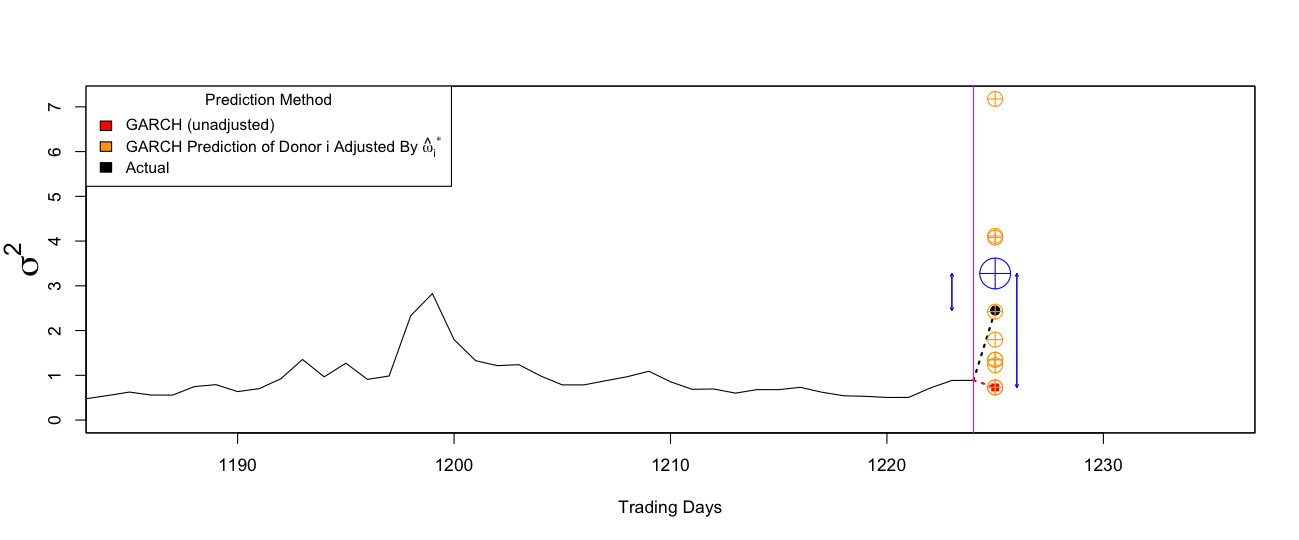
\includegraphics[width=\textwidth]{simulation_plots/motivating_piece_convex_combination.png}};
        % \draw[red,ultra thick,rounded corners] (7.5,5.3) rectangle (9.4,6.2);
        % \node[draw,text width=4.45cm] at (9.8,3.2) {$\textcolor{blue}{\hat\sigma^{2}_{adjusted} = \hat\sigma^{2}_{unadjusted} + \hat\omega^{*}}$ };
        % \node[draw,text width=2.62cm] at (14.8,2.8) {$\textcolor{blue}{\hat\omega^{*} = \sum^{n+1}_{i=2}\pi_{i}\hat\omega^{*}_{i}}$ };    
        
    \end{tikzpicture}
      \caption{The simulated time series experiences a volatility shock between trading days 1,656 and 1,657.  The GARCH prediction, in red, fails even to approach the volatility spike at $T^{*}+1$, as do several adjusted predictions, which are orange.  In contrast, the GARCH forecast adjusted by $\hat\omega^{*} = \sum^{n+1}_{i=2}\pi_{i}\hat\omega^{*}_{i} $, a convex combination of the estimated shocks in the donor pool, achieves directional correctness as well as a smaller absolute loss in its prediction.  The pink vertical line serves to indicate the adjustment of size $\hat\omega^{*}$ that allows the blue bullseye to approach more closely the ground truth.}    
      \label{fig:motivating_piece_convex_combination}
   
      \end{center}
    \end{figure}

  \subsection{A Primer on GARCH}
We define the log return of an asset between $t-1$ and $t$ as $r_{t} = \text{log}(\frac{P_{t}}{P_{t-1}})$, where $P_{t}$ denotes the price at time $t$.  The class of ARIMA($p,d,q$) models  \citep{box2013box} provides a framework for modeling the autoregressive structure of $r_{t}$.  These models assume a certain dependence structure between $r_{t}$ and $(r_{k})_{k\leq t}$, yet their errors --- often called innovations in the financial time series context due to how they represent the impact of new information --- are nevertheless assumed to be i.i.d. with mean zero and constant variance.  The ARCH \citep{engle1982autoregressive} and GARCH \citep{bollerslev1986generalized} models provide elegant alternatives to the homoskedasticity assumption.  In fact, the GARCH framework in its most basic form disregards $r_{t}$ and instead turns its interest to the series $r_{t}^{2}$ (once properly centered, i.e. after assuming a mean-model for returns).  

To that end, let $a_{t} = r_{t} - \mu_{t}$, where $\mu_{t}$ is the (potentially time-varying) mean of the log return series $r_{t}$.  We thus derive a mean-zero process $(a_{t})_{t\in\mathbb{N}}$ with the property that $\E[a^{2}_{t}] = \mrm{Var}[a_{t}]$.  Under the assumption of time-invariant volatility, the series $a_{t}^{2}$ should exhibit no significant autocorrelation at any lag $\ell\geq1$.  This assumption motivates tests for ARCH effects, that is, tests for the clustering of volatility.  These tests explore the alternative hypothesis that $\sigma_{t}^{2}$ is not only a time-varying parameter but furthermore a function of past squared residuals of the mean model.  In particular, the ARCH($m$) model is an autoregressive model in which $\sigma_{t}^{2}$ is a deterministic function of the past $m$ values of $r_{t}^{2}$.  The GARCH($m,s$) framework take this one step further by modeling $\sigma_{t}^{2}$ as a linear combination of the past $m$ values of $r_{t}^{2}$ and well as the past $s$ values of $\sigma_{t}^{2}$.  In functional form, a GARCH process (sometimes called a strong GARCH process \citep[p. 19]{francq2019garch}) is given by

\begin{align*}
&\sigma_{t}^{2} = \omega + \sum^{m}_{k=1}\alpha_{k}a^{2}_{t-k} + \sum_{j=1}^{s}\beta_{j}\sigma_{t-j}^{2}\\
&a_{t} = \sigma_{t}\epsilon_{t}\\
&\epsilon_{t} \simiid E[\epsilon_{t}]=0, Var[\epsilon_{t}] = 1\\
&\forall k,j, \alpha_{k},\beta_{j}\geq 0\\ 
&\forall t, \omega, \sigma_{t} > 0 \text { .} 
\end{align*}
Assuming further that $\sigma^{2}_{t}$ depends on a vector of exogenous covariates $\x_{t}$, we have a  GARCH-X$(m,s)$.  The volatility equation then becomes 

\begin{align}
\sigma_{t}^{2} = \omega+ \sum^{m}_{k=1}\alpha_{k}a^{2}_{t-k} + \sum_{j=1}^{s}\beta_{j}\sigma_{t-j}^{2} + \gamma^{T}\x_{t} \text{ .}\label{GARCH-X}
\end{align}

% https://latex-tutorial.com/matrices-in-latex/
% https://www.math-linux.com/latex-26/faq/latex-faq/article/how-to-write-matrices-in-latex-matrix-pmatrix-bmatrix-vmatrix-vmatrix

\subsection{Model setup}
\label{modelsetup}
We will suppose that a researcher has multivariate time series data $\y_{i,t} = (r_{i,t}$, $\x_{i,t}$), $t = 1,$ $\ldots,  T_i$, $i = 1, \ldots, n+1$, where $r_{i,t}$ is scalar and $\x_{i,t}$ is a vector of covariates such that $\x_{i,t}|\mathcal{F}_{i,t-1}$ is deterministic.  Suppose that the analyst is interested in forecasting the volatility of $r_{1,t}$, the first time series in the collection, which we will denote \textit{the time series under study}.  We require that each time series $\y_{i,t}$ is subject to an observed news event following $T^*_i \leq T_{i} + 1$ and before witnessing $T^*_i+1$.  We are implicitly leveraging the fact that financial assets are heavily-traded during market hours, yet only thinly traded (if traded at all) outside market hours.  In contrast, the arrival of market-moving news does not obey any such restrictions.  In light of the foregoing, we can denote our collection of GARCH-X volatility equations of interest using the following notation

\begin{align*}
&\sigma_{i,t}^{2} = \omega_{i} + \sum^{m_{i}}_{k=1}\alpha_{i,k}a^{2}_{i,t-k} + \sum_{j=1}^{s_{i}}\beta_{i,j}\sigma_{i,t-j}^{2} + \gamma_{i}^{T} \x_{i,t} \text{ }. \\
\end{align*}
Let $I(\cdot)$ be an indicator function.  Let $T_i$ denote the time length of the time series $i$ for $i = 1, \ldots, n+1$, and let $T_i^*$ denote the largest time index prior to the arrival of the news shock, with $T_i^* < T_i$, to ensure that there is at least one post-shock realization for each series $i$.  Let $\delta, \x_{i,t} \in \mathbb{R}^{p}$.  Let $\mathcal{F}_{i}$ with a single-variable subscript denote a univariate, time-invariant $\sigma$-algebra, and $\mathcal{F}_{i,t}$ denote the canonical product filtration for donor $i$ at time $t$.  Let $D^{return}_{i,t} = I(t \in \{T_i^* + 1,...,T_i^* + L_{i, return}\})$ and $D^{vol}_{i,t} = I(t \in \{T_i^* + 1,...,T_i^* + L_{i, vol}\})$, and let $L_{i,return},L_{i,vol}$ denote the lengths of the level and volatility shocks, respectively.  For $t= 1, \ldots, T_i$ and $i = 1, \ldots, n+1$, the model $\mc{M}_1$ is defined as 
\begin{align*}
  \mc{M}_1 \colon \begin{array}{l}
     \sigma^{2}_{i,t} = \omega_{i} + \sum^{m_{i}}_{k=1}\alpha_{i,k}a^{2}_{i,t-k} + \sum_{j=1}^{s_{i}}\beta_{i,j}\sigma_{i,t-j}^{2} + \gamma_{i}^{T} \x_{i,t} + \omega^{*}_{i,t}, \text{ }\\[.2cm]
     a_{i,t} = \sigma_{i,t}((1-D^{return}_{i,t})\epsilon_{i,t} + D^{return}_{i,t}\epsilon^{*}_{i}),\\[.2cm]
    \omega_{i,t}^{*} = D^{vol}_{i,t}[\mu_{\omega^{*}}+\delta^{T}\x_{i,T^{*}_{i}+1}+ u_{i,t}],
  \end{array}
  \end{align*}

with time-invariant error structure
  \begin{align*}
    \epsilon_{i,t} &\simiid \mc{F}_{\epsilon} \text{ with}  \; \mrm{E}_{\mc{F}_{\epsilon}}(\epsilon) = 0, \mrm{Var}_{\mc{F}_{\epsilon}}(\epsilon)  = 1,  \\
    \epsilon^{*}_{i,t} &\simiid \mc{F}_{\epsilon^{*}} \text{ with}  \; \mrm{E}_{\mc{F}_{\epsilon^{*}}}(\epsilon) = \mu_{\epsilon^{*}}, \mrm{Var}_{\mc{F}_{\epsilon^{*}}}(\epsilon^{*})  = \sigma^2_{\epsilon^{*}},  \\
    u_{i,t} & \simiid  \mc{F}_{u} \text{ with}  \; \mrm{Var}_{\mc{F}_{u}}(u) = \sigma^2_{u},\\
    \epsilon_{i,t} & \indep  \epsilon^{*}_{i,t}  \indep u_{i,t}.
    \end{align*}

    Let $\mc{M}_{0}$ denote the subclass of $\mc{M}_{1}$ models such that $\delta \equiv 0$.  Note that $\mc{M}_{0}$ assumes that nonzero shocks have no dependence on the covariates and are i.i.d. with $\E[ \omega^{*}_{i,t}]=\mu_{\omega^{*}}$, where the lack of indices $i$ or $t$ on $\mu_{\omega^{*}}$ indicates that it is shared across donors and is time-invariant. Models $\mc{M}_{1}$ and $\mc{M}_{0}$ parameterize changing dynamics after a shock is observed (when $t \geq T_i^*+1$ for each series $i$). It is important to note that our modeling setup will additionally suppose that $\x_{i,t}$ will be observed before $\sigma_{i,t}^2$ is observed. 
    
Note also the divergences from \cite{lin2021minimizing}.  As already established, the model presented here is intended to account for ARCH effects.  Additionally, here we also diverge by modeling the shocks $\omega^{*}_{i,t}$ as time-varying quantities obeying a mixture distribution.  In particular, prior to and after the shock, the  $\omega^{*}_{i,t}$  are uniformly zero.  During the shock, i.e. from $T^{*}_{i}+1$ through $T^{*}_{i}+L^{vol}_{i}$, the $\omega^{*}_{i,t}$ are distributed i.i.d, with a core signal component that depends solely on the unknown parameter $\delta$ and the observable vector $\x_{i,T_{i}^{*}+1}$.  Wherever necessary, to distinguish the two distributions that make up the shock distribution, we use the term \textit{nonzero shocks} to refer to the shocks that are not uniformly zero.  

The nonzero shocks each include an idiosyncratic noise term that varies across time and donors.  This feature allows the nonzero shocks to exhibit some variation as the shock progresses, even within a single donor.  The noise term could be modeled with additional complexity, including serial correlation, or could exhibit determinstic or stochastic decay throughout the shock period, proportional to a deterministic or stochastic function of time, or could peak somewhere in the middle of the shock period.  Each of these ideas might correspond to some particular, realistic feature of the world.

The model $\mc{M}_1$ is defined by a volatility equation and mean equation, as is any GARCH model.  The decision to model the volatility shock $\omega^{*}_{i,t}$ as an additive random effect is consistent with our setup.  However, the decision to model the level effect $\epsilon^{*}_{i,t}$ as a temporary rupture in the otherwise i.i.d. sequence of innovations $\epsilon_{i,t}$ may not be intuitive.  One way of arguing for this choice is that, in a discrete time series model, if we assume the arrival of news in the time between $T_{i}^{*}$ and $T_{i}^{*}+1$, we do not have an easy way to express a conditional distribution of the innovation $\epsilon_{i,T_{i}^{*}+1}$ given the arrival of information.  Using $\epsilon^{*}_{i,t}$ thus breaks this impasse.  This justification also explains why we do not parameterize the level shock at $T_{i}^{*}+1$ as a sum of two shocks, $\epsilon_{i,T_{i}^{*}+1}$ and $\epsilon^{*}_{i,T_{i}^{*}+1}$, which would represent the level shock as generated by two independent sources of stochasticity. While we want to model the level shocks at $T_{i}^{*}+1$ as potentially large in absolute value, we also want to retain the property of a unitary source of noise.


\section{Methodology for Similarity-based Parameter Correction}

We now introduce how a researcher can carry out predictions via distance-based weighting.  The first step is to gather the $p$ covariates that will parametrize a change in dynamics to model $\mc{M}_1$ and will represent the $p$-dimensional space in which weights are generated.  This set of covariates parameterizes the shock to $\sigma^2_{i,t}$  of magnitude $\omega^*_{i,t}$ in model $\mc{M}_{1}$ above.  Let $\textbf{V}_{t} \in \mathbb{R}^{p \times n}$ be formed with columns $\x_{i,t}$, $i = 2,\ldots,n+1$.  Without loss or generality, let the indices of each $\x_{i,t}$ be shifted and arranged such that $\textbf{V}_{T^{*}+1}$ has as columns $\x_{2,T_{2}^{*}+1},...,\x_{n+1,T_{n+1}^{*}+1}$.  Formally, in vector notation, the donor shocks are given by $\vec{\omega}_t = \vec{\mu}_{\omega^{*}} + \delta^{T}\textbf{V}_{t} + \vec{u}_{t}$, 
    where were have suppressed the $D^{vol}_{i,t}$ notation for simplicity.  %The covariate set could take the form of a $p \times n$ matrix including realized volatility and implied volatility, as well the volume of traded assets on any day preceding the shock.  Covariates chosen for inclusion in a given volatility profile may be levels, log differences in levels, percentage changes in levels, or absolute values thereof, among many choices.
    Ideally, $\textbf{V}_{t}$ will display `balance' in that $p$ covariates exist for each of the $n$ donors.  In practice, missing values, corrupted values, or unacceptably extreme or noisy estimates may necessitate some sort of matrix completion, a problem that we do not tackle in this work.  

\subsection{Forecasting}

We now turn to the next section, where $\textbf{V}_{t}$ is employed in a procedure to arrive at a forecast adjustment. For illustration, we present two one-step-ahead forecasts for the time series under study. The first is the unadjusted GARCH forecast. The second is the adjusted forecast, which differs by the additive term $\hat\omega^{*}$ that is computed via our distance-based weighting procedures.  These forecasts are: 

\begin{align*}
  %\text{Forecast 1: } 
  & \hat\sigma^{2}_{unadjusted,T_{1}^{*}+1} = \hat\E[\sigma^{2}_{1,T_{1}^{*}+1}|\mathcal{F}_{T_{1}^{*}}] && = && \hat\omega_{1} + \sum^{m_{1}}_{k=1}\hat\alpha_{1,k}a^{2}_{1,T_{1}^{*}+1-k} + \sum_{j=1}^{s_{1}}\hat\beta_{1,j}\sigma_{1,T_{1}^{*}+1-j}^{2} + \hat\gamma_{1}^{T} \x_{1,T_{1}^{*}+1},\\
  %\text{Forecast 2: } 
  & \hat\sigma^{2}_{adjusted, T_{1}^{*}+1} = \hat\E[\sigma^{2}_{1,T_{1}^{*}+1}|\mathcal{F}_{T_{1}^{*}}] + \hat\omega^{*} && = && \hat\omega_{1} + \sum^{m_{1}}_{k=1}\hat\alpha_{1,k}a^{2}_{1,T_{1}^{*}+1-k} + \sum_{j=1}^{s_{1}}\hat\beta_{1,j}\sigma_{1,T_{1}^{*}+1-j}^{2} + \hat\gamma_{1}^{T} \x_{1,T_{1}^{*}+1} + \hat\omega^{*} \text{ .}
\end{align*}

Note that GARCH models can be parameterized as ARMA models on the squares of the scalar time series $a_{i,t}^{2}$ \citep[][p. 18, p. 46]{tsay2005analysis,francq2019garch}, assuming that $a_{i,t}$ satisfies fourth-order stationarity.  This fact matters for forecasting because the $h$-step-ahead forecasting function for a GARCH model is, just like for an ARMA model, the conditional expectation function, $\mathbb{E}[ \sigma^{2}_{i,T_{i}^{*}+h} | \mathcal{F}_{T_{i}^{*}}]$, or practically speaking, the estimate thereof, $\hat{\mathbb{E}}[ \sigma^{2}_{i,T_{i}^{*}+h} |\mathcal{F}_{T_{i}^{*}}]$ \citep{zivot2009practical}.  Here we have presented one-step-ahead forecasts for a GARCH-X($m,s$).  For $h=2,3,4,...$, the conditional expectation is computed recursively, as is standard for iterative autoregressive forecasts. Note that $h$-step-ahead predictions will require, of course, some reasonable idea about the length of time for which the adjustment quantity $\hat\omega^{*}$ should be included.  Addtionally, if $\x_{1,t}$ is used as an exogenous regressor in order to estimate $\gamma_{1}$, then strictly speaking, $\x_{1,t+h}|\mathcal{F}_{t}$ must be deterministic.   In practice, it may be acceptable that $\x_{1,t+h}|\mathcal{F}_{t}$ is merely well-estimated. Thus for simplicity of exposition, we will focus on the one-step-ahead forecast unless stated otherwise.

\subsection{Excess Volatility Estimators}
    \label{Excess Volatility Estimators}
   
    The problem of aggregating estimated donor shocks begins with the data constraints.  Let us first introduce useful notation.  Let $\hat\omega^{*}_{i,*}$ denote the shock estimate for donor $i$ that is obtained via fixed effect estimation over time points $T_{i}^{*}+1,...,T_{i}^{*}+L_{i,vol}$.  That estimation procedure is justified by the assumption that at each nonzero shock point, the shocks will differ but will be equal in distribution.  
    
    Taking the estimated shocks as a given, we observe the pair $(\{\hat\omega^{*}_{i,*}\}^{n+1}_{i=2},\{\textbf{v}_{i}\}^{n+1}_{i=2})$.  Let $\Delta^{n-1} = \{\pi \in \mathbb{R}^n: \sum_{i=1}^n \pi_i = 1, \pi_i \geq 0, i = 1,...,n\}$.  We wish to recover weights $\{\weight_{i}\}^{n+1}_{i=2} \in \Delta^{n-1}$ leading to favorable forecasting properties.  These weights are used to define and compute an aggregate shock estimate 
\begin{equation} \label{adjustment}
	  \hat\omega^{*} = \sum^{n+1}_{i=2}\weight_{i}\hat\omega^{*}_{i,*},
\end{equation}
    which will be taken to be our forecast adjustment term.  Since the weights $\{\weight_{i}\}_{i=2}^{n+1}$ are computed using $\mathcal{F}_{T^{*}_{i}}$, the set $\{\weight_{i}\}_{i=2}^{n+1}$ is deterministic and observed, $\textit{modulo}$ any stochastic ingredient in the numerical methods employed to approximate $\x_{1,T_{1}^{*}+1}$ using a convex combination of donor covariates.  We say more about the properties of the shocks $\omega^{*}_{i,T_{i}^{*}+1},...,\omega^{*}_{i,T_{i}^{*}+L^{vol}_{i}}$ in section $\ref{SVF_properties}$. 

    Following \citet{abadie2003economic,abadie2010synthetic,lin2021minimizing}, let $\|\cdot\|_{\textbf{S}}$ denote any semi-norm on $\mathbb{R}^{p}$, and define
    \begin{align*}
    \{\pi\}_{i=2}^{n+1} = \argmin_{\pi}\|\x_{1,T_{1}^* + 1} - \V_{T^* + 1}\pi\|_{\textbf{S}}. 
    \end{align*}
In the forecast combination literature, it is of interest whether the weights employed to aggregate forecasts strive toward and meet various optimality criteria \citep{timmermann2006forecast,wang2023forecast}.  In our endeavor, there are at least two senses of optimal weights that one might be interested in.  First, we can think of optimal weights as a set $\{\weight_{i}\}_{i=2}^{n+1}$ such that $\omega_{1} = \sum^{n+1}_{i=2}\weight_{i}\hat\omega_{i,*}$, i.e., $\omega_{1}$ is recovered perfectly, as it belongs to convex hull of the estimated shocks. However, $\omega_{1}$ is never revealed to the practitioner, and hence there is no way of verifying the extent to which this condition is satisfied.

A more promising aim is finding weights such that $\textbf{v}_{1} = \sum^{n+1}_{i=2}\weight_{i}\textbf{v}_{i,T_{1}^{*}+1}$, meaning that the covariates of the time series under study lies within the convex hull of the donor covariates.  This condition underwrites asymptotic results in \citet{abadie2010synthetic}, and the intuition there extends to this work: if the shock is parameterized by an affine function of covariates, then finding a linear combination that recreates the shock should serve us well.  Because the method proposed uses a point in $\Delta^{n-1}$, it is important to head-off possible confusion.  What we are proposing is not a forecast combination method.  What we are aggregating and weighting (not combining) are subcomponents of forecasts, not forecasts themselves.  Moreover, from a broader perspective, forecast combination is an inapt term for what is being proposed here.  First, the donor time series do not provide forecasts, nor would forecasts be needed for random variables that have already been realized.  Second and more fundamentally, the theoretical underpinnings of forecast combination, while diverse \citep{wang2023forecast}, are distinct from the setting presumed in this work.

Supposing that we can define optimal weights, then uniqueness may still be a concern. \cite{lin2021minimizing} discuss sufficient conditions for uniqueness as well as the implications of non-uniqueness.  \cite{abadie2022synthetic} invoke the Carath\'eodory Theorem to argue for the sparseness of the weight vector.  We make additional comments as well. $(\mathbb{R}^{n}, \|\cdot\|)$ is a Chebyshev space, and hence for any element x and any convex set $C\subset \mathbb{R}^{n}$, there exists a unique element $y\in C$ that minimizes $\|x-y\|$.  However, the pre-image of $y$ with respect to a particular operator and constraint set might not be unique.  Let $p', n'$ denote the number of linearly independent rows of $\V_{t}$ and linearly independent columns of $\V_{t}$, respectively.  Let col($\cdot$) denote the column space of a matrix, and let Conv($\cdot$) denote the convex hull of a set of column vectors. Then the following table is useful for categorization of when a perfect fit and uniqueness prevail: \\

    \begin{center}
      \begin{tabular}{ | m{3em} | m{7cm}| m{7cm} | } 
        \hline
        & $\textbf{v}_{1}\in \text{Conv}(\text{col}(\V_{t}))$ & $\textbf{v}_{1} \notin \text{Conv}(\text{col}(\V_{t}))$\\ 
        \hline
        $p' \geq n'$ & Perfect fit; minimizer unique & Fit not perfect; minimizer unique \\
        \hline
        $p' < n'$ & Perfect fit; minimizer not necessarily unique, Carath\'eodory Theorem applies& Fit not perfect; minimizer not necessarily unique, Carath\'eodory Theorem applies \\ 
        \hline
      \end{tabular}
      \end{center}
      
It should be noted, however, that even when the minimizer is unique, finding that unique minimizer will require numerical methods.  In the event that one's preferred numerical optimization routine fails to arrive at a single solution on the simplex in repeated runs of the algorithm, some sort of forecast combination might be advised.  We discuss forecast combination later in this paper in the context of robustifying against misspecification.

On the questions of convex geometry and convex optimization, comparison with least-squares estimation is also illustrative.  Consider least-squares estimation for the $p$-vector $\delta$ in the shocks $\omega^{*}_{i,t}$:

\begin{align*}
 \hat\omega^{*}_{OLS} =\argmin_{\delta}\|\hat{\omega}^{*} - \delta^{T}\textbf{V}_{T^{*}+1}\|^{2}_{2},
\end{align*}
where $\textbf{V}_{T^{*}+1}$ could include an adjoined row $\textbf{1}_{n}$, in order to estimate the locator parameter of the shock.  One problem is that this optimization problem is an optimization problem over $p$-vectors $\delta$ --- over linear combinations of the covariates, whereas what we seek is an $n$-vector --- a linear combination of donors.  Additionally, there is no guarantee that $\hat\omega^{*}_{OLS} = \hat{\delta}_{OLS}^{T}\x_{1,T^{*}+1}$ would perform poorly, but given the small number of donors supposed in our setting, it is risky.  Last, and perhaps most challenging for the least-squares estimate, $\hat{\delta}_{OLS}^{T}$ faces the usual requirement of more donors than linearly-independent covariates, and that may not often be easy to satisfy in our setting.

\subsection{Ground Truth Estimators}
    \label{Ground Truth Estimators}
    
    The time-varying parameter $\sigma^{2}_{t}$ is a quantity for which even identifying an observable effect in the real world is far more challenging.  In this work, we use a common estimator of the variance called realized volatility (RV), one which has the virtue of being ``model-free'' in the sense that it requires no modeling assumptions \citep{andersen2010stochastic}.  The realized variance itself can be decomposed into the sum of a continous component and a jump component, with the latter being less predictable and less persistent \citep{andersen2007roughing}, cited in \citet{de2006forecasting}, two factors that further motivate the method employed herein.
    
    Suppose we examine $K$ units of of time, where each unit is divided into $m$ intervals of length $\frac{1}{m}$.  We adapt the notation of \citet{andersen2008realized}. Let $p_{t} = \log{P_{t}}$, and let $\tilde{r}(t,\frac{1}{m}) = p_{t} - p_{t-\frac{1}{m}}$.  Suppressing the $i$ index, we estimate the variance the log return series using Realized Volatility of the $K$ consecutive trading days that conclude with day $t$, denoted $RV_{t}^{K,m}$, using    
   \begin{align*}
    RV_{t}^{K,m} = \frac{1}{K}\sum^{Km}_{v=1}\tilde{r}^{2}(v/m,1/m),
   \end{align*}
    where the $K$ trading days have been chopped into $Km$ equally-sized blocks.

    Assuming that the $K$ units $\tilde{r}(t, 1) = p_{t} - p_{t-1}$ are such that $\tilde{r}(t, 1) \simiid N(\mu, \delta^{2})$, it is easily verified that $\E[RV^{K,m}] = \frac{\mu^{2}}{m} + \delta^{2}$, which is a biased but consistent estimator of the variance.  We will proceed using $m = 77$, corresponding to the 6.5-hour trading day chopped into 5-minute blocks, with the first block omitted in order to ignore unusual trading behavior at the start of the day. Other sensible choices for $m$ can replace our specification if desired.

\subsection{Loss Functions}\label{loss_function}

We are interested in point forecasts for $\sigma^{2}_{1,T_{1}^{*}+h}|\mathcal{F}_{T_{1}^{*}}$, $h=1,2,...,$ the $h$-step ahead conditional variance for the time series under study.  Let $L^{h}$ with the subscripted pair $\{$prediction method, ground truth estimator$\}$, denote the loss function for an $h$-step-ahead forecast using a given prediction function and ground truth estimator.  For example, the $h$-step-ahead MSE when forecasting from time $t$ using our method and using Realized Volatility as the ground truth is

$$ \text{MSE}^{h}_{\text{aggregated predictor, RV}} = (\hat\sigma^{2}_{\text{aggregated predictor},t+h} - \hat\sigma^{2}_{RV,t+h})^{2}$$
Also of interest in absolute percentage error for an $h$-step-ahead forecast, defined as

\[ 
\text{APE}^{h}_{\text{method, ground truth}} = \frac{|\hat\sigma^{2}_{\text{method},t+h} - \hat\sigma^{2}_{\text{ground truth},t+h}|}{\hat\sigma^{2}_{\text{ground truth},t+h}}
\]
Finally, we introduce the QL (quasi-likelihood) Loss \citep{brownlees2011practical}:

\[ 
\text{QL}^{h}_{\text{method, ground truth}} = \frac{\hat\sigma^{2}_{\text{ground truth},t+h}}{ \hat\sigma^{2}_{\text{method},t+h}} - \log{\frac{\hat\sigma^{2}_{\text{ground truth},t+h}}{ \hat\sigma^{2}_{\text{method},t+h}}} -1 \text{ .}
\]
What distinguishes QL Loss is that it is multiplicative rather than additive.  This has benefits, both practical and theoretical.  As \citet{brownlees2011practical} explain, the technical properties of the QL Loss allow researchers to compare forecasts across heterogeneous time series, whereas additive loss functions like MSE unfairly penalize forecasts made under market turbulence.  For this reason and others, we proceed to evaluate the method, both in simulations and real data examples, using the QL loss.

\section{Properties of Volatility Shocks and Shock Estimators}\label{SVF_properties}

In this section we will provide estimation properties for our shock  estimator \eqref{adjustment} and our adjusted forecast. These results will be with $m_i = s_i = 1$, for all $i = 1,\ldots,n+1$ in model $\mc{M}_1$ unless otherwise stated, i.e. a GARCH(1,1) model with additional parameterizations for shocks. Note that the dual level-volatility shock in $\mc{M}_1$ has a marginal effect on the conditional variance $\sigma^{2}_{i,t}$ that reflects the geometric decay of innovations in autoregressive models.  As usual, assume $\alpha+\beta < 1$.  Furthermore, assume that both the volatility shock and the level shock are of length one only, and consider a circumstance with no exogenous covariate $\x_{i,t}$, except in the conditional shock distribution. Assume also that $r\geq 2$, which is necessary in order to isolate the effects of the level shock $\epsilon^{*}_{i,t}$.  Then
\begin{align}
\sigma^{2}_{i,T_{i}^{*}+r+1} | \mathcal{F}_{T_{i}^{*}+r} & = \omega_{i} + \alpha_{i} a_{T_{i}^{*}+r}^{2} + \beta_{i}\sigma^{2}_{i,T_{i}^{*}+r} \label{eq0}\\
& = \omega_{i} + \alpha_{i}(\sigma_{i,T_{i}^{*}+r}\epsilon_{T_{i}^{*}+r})^{2} + \beta_{i}\sigma^{2}_{i,T_{i}^{*}+r}\notag \\
& = \omega_{i} + \sigma^{2}_{i,T_{i}^{*}+r}(\alpha_{i} (\epsilon_{T_{i}^{*}+r})^{2} + \beta_{i}) \text{ .}\notag 
\end{align}

In Equation \eqref{eq0}, observe that $\omega_{i,T_{i}^{*}+1}^{*}$ and $\epsilon^{*}_{i,T_{i}^{*}+1}$ 
each appear at most once, through the term $\sigma^{2}_{T_{i}^{*}+r}$.  This might lead one to 
suspect  geometric decay of the shocks $\omega_{i,T_{i}^{*}+1}^{*}$ and $\epsilon^{*}_{i,T_{i}^{*}+1}$.  
Such a suspicion is easier to justify by examining the conditional expectation of the variance, 
$\mathbb{E}[ \sigma^{2}_{i,T_{i}^{*}+r+1} |\mathcal{F}_{T_{i}^{*}+r}]$, which also happens to be the principal forecasting tool for a GARCH model \citep{zivot2009practical}.  Indeed, if we assume unit variance for all $\epsilon_{i,t}$ except, of course, $\epsilon^{*}_{i,t}$, then we have

\begin{align*}
\mathbb{E}[ \sigma^{2}_{i,T_{i}^{*}+r+1} |\mathcal{F}_{T_{i}^{*}+r}] & = \mathbb{E}[\omega_{i} + \alpha a_{T_{i}^{*}+r}^{2} + \beta\sigma^{2}_{i,T_{i}^{*}+r} |\mathcal{F}_{T_{i}^{*}+r}] \\
& = \omega_{i} + \mathbb{E}[\alpha(\sigma_{i,T_{i}^{*}+r}\epsilon_{T_{i}^{*}+r})^{2} |\mathcal{F}_{T_{i}^{*}+r}] + \beta\sigma^{2}_{i,T_{i}^{*}+r} \\
& = \omega_{i} + \alpha\sigma_{i,T_{i}^{*}+r}^{2} + \beta\sigma^{2}_{i,T_{i}^{*}+r} \tag{Due to the unit variance assumption}\\
& = \omega_{i} + \sigma^{2}_{i,T_{i}^{*}+r}(\alpha + \beta) \text{ .} 
\end{align*}
By repeated substitution, in conditional expectation, the shock belongs to the equivalence class $\mathcal{O}((\alpha+\beta)^{r})$.  We generalize this observation in the following proposition.

\begin{prop}\label{decay_prop}
Let $a_{t}$ be a mean-zero time series obeying a GARCH(1,1) specification with unit-variance errors, all prior to the arrival of a volatility shock of length $L_{\text{vol}} \geq 1$ and level shock of length $L_{\text{return}}\geq 1$ at some time $T^{*}+1$.  Then for any $r$ such that $r \geq \text{max}\{L_{i, vol},L_{i, level}\} + 1$, 
\begin{align*}
\mathbb{E}[ \sigma^{2}_{i,T_{i}^{*}+r+1} |\mathcal{F}_{T_{i}^{*}+r}] & = \omega_{i} + (\alpha + \beta)\sigma^{2}_{i,T_{i}^{*}+r}.
\end{align*}
\end{prop}


In other words, for a GARCH(1,1), once two time points removed from the longest shock length, the volatility shock and level shock can be subsumed into one.  However, prior to being two time points removed, there is no such guarantee.  For example, one can take $r = 1$ and level shock of length at least 1 to see that 
\begin{align*}
\mathbb{E}[ \sigma^{2}_{i,T_{i}^{*}+2} |\mathcal{F}_{T_{i}^{*}+1}] & = \mathbb{E}[\omega_{i} + \alpha a_{T_{i}^{*}+1}^{2} + \beta\sigma^{2}_{i,T_{i}^{*}+1} |\mathcal{F}_{T_{i}^{*}+1}] \\
& = \omega_{i} + \mathbb{E}[\alpha(\sigma_{i,T_{i}^{*}+r}\epsilon^{*}_{T^{*}+1})^{2} |\mathcal{F}_{T_{i}^{*}+1}] + \beta\sigma^{2}_{i,T_{i}^{*}+1} \\
& = \omega_{i} + \alpha\sigma^{2}_{i,T_{i}^{*}+1}(\mu^{2}_{\epsilon^{*}} + \sigma^{2}_{\epsilon^{*}}) + \beta\sigma^{2}_{i,T_{i}^{*}+1} \\
& = \omega_{i} + \sigma^{2}_{i,T_{i}^{*}+1}(\alpha(\mu^{2}_{\epsilon^{*}} + \sigma^{2}_{\epsilon^{*}}) + \beta)\text{,}
\end{align*}
where $(\alpha(\mu^{2}_{\epsilon^{*}} + \sigma^{2}_{\epsilon^{*}}) + \beta)$ may be greater than 1, permitting explosive behavior, at least in the short term.  After both shocks have been exhausted, their influence disappears quickly.  This short-memory effect has implications for the method being developed herein.  First, there may be different risks associated with overestimating and underestimating level shock and volatility shock lengths.  Therefore, estimation of effects among the donors should err on the side of underestimating, not overestimating, the length of the max shock, since overestimation of the shock length brings with it the risk of underestimating $\omega^{*}_{i,t}$.  Second, a practitioner of the method needs some idea of how long the the respective shocks in the time series under study might last.  There are couple of obvious strategies: take all the donors, and over all the donor shock lengths, take the minimium.  Alternatively, one could take the maximum.

\subsection{Consistency of the shock estimators}

The estimators $\hat\omega^{*}_{i,t}$ in \eqref{adjustment} are central to our forecast adjustment strategy.  Here we show that the quantities $\hat\omega^{*}_{i,t}$ possess an important asymptotic property that bolsters that overall reliability of the method proposed herein.

\begin{prop}\label{omega_consistency}
Assume
\begin{enumerate}
  \item For each $i$, $\{a_{i,t}\}_{t=0,...,T_i}$ obeys a GARCH-X($m,s$), as laid out in Equation $\eqref{GARCH-X}$, with volatility shocks found in $\mc{M}_{1}$, where $T_i$ is the length of the $i$th series.
  \item For each $i, \{D^{vol}_{i,t}\omega_{i,t}^{*}\}_{t=0,...,T_i}$ is potentially non-zero at $\{T^{*}_{i}+1,... ,T^{*}_{i}+L_{i}^{vol}\}$, $\omega_{i,T_{i}^{*}+1}^{*}\equiv...\equiv\omega_{i,T_{i}^{*}+L_{i}^{vol}}^{*}$, and zero otherwise, where the arrival of $T_{i}^{*}$ is governed by a time-invariant distribution on $\{a_{i,t}\}_{t=0,...,T_i-1}$, and both the arrival and conclusion of the shock is observable by the researcher. \label{stationarity_of_omega_i_t}
  \item The conditions in Assumption 0 of \citet{han2014asymptotic} hold.
\end{enumerate}
Then for any $i, 1\leq i \leq n+1$, and for any $r, 1\leq r \leq L_{i}^{vol}$, $\hat\omega_{i,T_{i}^{*}+r}^{*} \overset{p}{\longrightarrow} \omega_{i,T_{i}^{*}+r}^{*}$ as $t\rightarrow\infty$.  Additionally, $\hat\omega_{i,*}^{*} \overset{p}{\longrightarrow} \omega_{i,T_{i}^{*}+r}^{*}$ as $t\rightarrow\infty$.  That is, whether estimated  individually or collectively, the nonzero shock estimators are consistent.
\end{prop}

\begin{lem}\label{lemma_ref}
  Under assumption \ref{stationarity_of_omega_i_t}, for each $i, i=1,...,n+1$,  $\{\omega_{i,t}^{*}\}_{t=0,...,T_i}$ is a strictly stationary series.
\end{lem}

\subsection{Consistency of the Conditional Forecast Function}

Having established the consistency of the estimators $\hat\omega^{*}_{i,T_{i}^{*}+1}$, we extend that result to prove the consistency of the conditional forecast function itself.

  \begin{prop}\label{sigma_consistency}
    Assume
    \begin{enumerate}
      \item All conditions listed in Proposition \ref{omega_consistency}.
      \item There exist weights $\{\pi_{i}\}_{i=2}^{n+1}$ such that $\textbf{v}_{1,T_{1}^{*}} = \sum^{n+1}_{i=2}\weight_{i} \textbf{v}_{i,T_{i}^{*}}$.
     \end{enumerate}
  Then for any $r$, $1\leq r \leq L_{i}^{vol}$, $\hat\sigma^{2}_{adjusted,T_{i}^{*}+r}\overset{p}{\longrightarrow}\sigma^{2}_{1,T_{i}^{*}+r}$ as $t\rightarrow\infty$. 
  \end{prop}

\subsection{Asymptotic Loss}

We now evaluate the loss and risk of our method under two scenarios: first, under arbitrary distribution of $\sigma^{2}_{t+1}$, and then second, under the assumption that the data-generating process is correctly specified.  For simplicity, we suppress the index $i$ on all quantities.

For a 1-step-ahead forecast of $\sigma^{2}_{t+1}$ where $t=T^{*}$, consider the difference 
\begin{align}
  & QL(\hat\sigma_{unadjusted,t+1}^{2},\sigma^{2}_{t+1})-QL(\hat\sigma^{2}_{adjusted,t+1},\sigma^{2}_{t+1})\notag \\
   & =(\frac{\sigma_{t+1}^{2}}{\hat\sigma^{2}_{unadjusted,t+1}} - \log{\frac{\sigma_{t+1}^{2}}{\hat\sigma^{2}_{unadjusted,t+1}} } - 1) - (\frac{\sigma_{t+1}^{2}}{\hat\sigma^{2}_{adjusted,t+1}} - \log{\frac{\sigma_{t+1}^{2}}{\hat\sigma^{2}_{adjusted,t+1}}} - 1)\notag\\
   & = \frac{\sigma_{t+1}^{2}}{\hat\sigma^{2}_{unadjusted,t+1}} - \frac{\sigma_{t+1}^{2}}{\hat\sigma^{2}_{adjusted,t+1}}+ \log{\frac{\hat\sigma^{2}_{unadjusted,t+1}}{\hat\sigma^{2}_{adjusted,t+1}}}\notag\\
   & = \frac{\sigma_{t+1}^{2}(\hat\sigma^{2}_{adjusted,t+1}-\hat\sigma^{2}_{unadjusted,t+1})}{\hat\sigma^{2}_{adjusted,t+1}\hat\sigma^{2}_{unadjusted,t+1}} + \log{\frac{\hat\sigma^{2}_{unadjusted,t+1}}{\hat\sigma^{2}_{adjusted,t+1}}}\label{QL Loss toy example} \text{ .}
\end{align}
For simplicity, we work with a GARCH(1,1) that experiences a volatility shock at a single time point for which we would like to provide a point forecast.  Then (\ref{QL Loss toy example}) can be expressed as
\begin{align*}
   &\frac{\sigma^{2}_{t+1}\hat\omega^{*}_{t+1} }{\hat\sigma^{2}_{adjusted,t+1}\hat\sigma^{2}_{unadjusted,t+1}} + \log{\frac{\hat\omega + \hat\alpha a_{t}^{2} + \hat\beta\sigma_{t}^{2}}{\hat\omega + \hat\alpha a_{t}^{2} + \hat\beta\sigma_{t}^{2} + \hat\omega^{*}_{t+1}}}.
\end{align*}\label{QL Loss Consistency - GARCH(1,1)}
It is easily verified that as $\hat\omega^{*}_{t+1} \rightarrow 0^{+}$, the difference in the losses goes to zero.  On the other hand, as $\hat\omega^{*}_{t+1}$ becomes large, the difference in the losses turns negative, with the lesson being that $\hat\omega^{*}_{t+1}$ must be in appropriate proportion to $\sigma^{2}_{t+1}$ in order for the adjusted forecast to outperform the unadjusted forecast.  This explains why it is so important to avoid using a naive adjustment estimator, $\overline{\omega^{*}}$, the arithmetic mean of the estimated shocks.  We conclude this section with a broader result. 

\begin{prop}\label{asymptotic_consistency}
Assume the conditions in Propositions $\ref{omega_consistency}$ and $\ref{sigma_consistency}$.  Let $1\leq i\leq n+1$.  Then as $t\rightarrow \infty$,
$$QL(\hat\sigma_{unadjusted,t+1}^{2},\sigma^{2}_{t+1})-QL(\hat\sigma^{2}_{adjusted,t+1},\sigma^{2}_{t+1}) \overset{p}{\longrightarrow} \frac{\omega_{i,t+1}^{*}}{\sigma^{2}_{i,t+1}-\omega_{i,t+1}^{*}} + \log{\frac{\sigma_{i,t+1}^{2}-\omega_{i,t+1}^{*}}{\sigma_{i,t+1}^{2}} } \geq 0.$$
Hence, a correctly specified $\mc{M}_1$ model will outperform the unadjusted forecast asymptotically.
\end{prop}

\section{Numerical Examples}

In this section, we demonstrate the effectiveness of the proposed method using Monte Carlo simulations.  All simulations will use $\mc{M}_1$ volatility models and $\mc{M}_0$ models on the returns, i.e. $  D^{return}_{i,t} \equiv 0$ for each $i$ and each $t$.  We first explain the parameters to be varied, the parameters that remain fixed, and the behavior we expect to observe.  For our purposes, a parameter is defined to be fixed whenever it does not vary across any of the simulations performed, and conversely, a parameter is varying whenever it varies across at least two simulations performed. The overarching story told by the simulations is that our method performs well as the magnitude of the signal in the shock grows relative to the variance of the idiosyncratic noise term of the shock. 
%For brevity, we refer to this as the signal-to-noise phenomenon.  However, this phenomenon is complicated somewhat by at least two nuances: additional parameters must be in place and properly sized in order to enable to signal-to-noise phenomenon, and second, certain hurdles must be met in the size of those additional parameters before the signal-to-noise story can be seen.  In short, interaction effects abound, with non-linearities as well.

  \subsection{Fixed Parameters}
Each simulation, $i=1,...n+1$ is a GARCH(1,1) process of length $T_{i}$ chosen randomly from the set of integers $\{756,...,2520\}$, corresponding to approximately 3-10 years of daily financial data.  We fixed the intercept of the processes at the $\textit{garchx}$ package default of $\omega = .2$ \citep{RePEc:pra:mprapa:100301}.  We also use the values $\alpha=.1, \beta = .82$, corresponding to a GARCH process with greater influence from past values of $\sigma^{2}_{i,t}$ than past values of $a^{2}_{i,t}$.


  \subsection{Varying Parameters}
  We vary exactly five parameters: $\mu_{V}, \sigma_{V}, \mu_{\delta}, \mu_{\omega^{*}}, \sigma_{u}$, each of which is critical to evaluating the method's responsiveness to changing conditions in the shock distribution. $\mu_{V}, \sigma_{V}$ govern the elements of the covariates. $\mu_{\delta}$ interacts with $\textbf{V}_{t}$ via the dot-product operation, of course.  $\mu_{\omega^{*}}$ is a location parameter for the volatility shock, and $\sigma_{u}$ is the standard deviation of the volatility shock.
  
  We add an important note about the parameter $\mu_{\delta}$, which governs a vector $\delta$ of length $p$ with elements that increase monotonically in proportion to $1,...,p$, after which they are scaled by the factor $\frac{2\cdot\mu_{\delta}}{p(p+1)}$, so that a randomly selected entry of the vector has mean $\mu_{\delta}$.  The heterogeneity of the entries in $\delta$ is critical to simulating the plausible heterogeneity that will exist in the random effects structure.  Absent a heterogeneous vector $\delta$, the shock would not vary systematically with regard to each variable in the covariate vector.  Such a setup would fail to approximate the realities of financial markets.

\subsection{Evaluative Framework and Monte Carlo Results}
Consistent with our evaluative framework declared in \ref{loss_function}, we compare adjusted and unadjusted forecasts using QL Loss, calculating the fraction of the simulations in which the adjusted forecast yields a QL Loss no smaller than that of the unadjusted forecast.  The simulations fall into three broad categories, which we will denote \textbf{Signal and Noise} (displayed in Figure \ref{fig:signoise}), \textbf{Interaction between Signal and Volatility Profile Means} (displayed in Figure \ref{fig:sig_volprof}), and lastly, \textbf{Interaction between Shock Intercept and Shock Noise} (displayed in Figure \ref{fig:intercept_noise}).  

The first category plots two parameters of the shock equation, $\mu_{\delta}$ and $\sigma_{u}$, in grids while increasing the mean of the covariate vectors $\x$ over three plots.  Recall that $\delta$ is a parameter shared between donors, whereas each vector $\x_{i,t}$ in $\V_{i,t}$ is i.i.d. multivariate normal.  In Figure \ref{fig:sim_1}, we see very little variation across the grid.  However, in Figures \ref{fig:sim_2} and \ref{fig:sim_3}, where $\mu_{v}$ is increased, we observe an expected phenomenon: for any fixed column of the plots, the performance of the adjusted forecast improves with increasing $\mu_{\delta}$.  A somewhat subtler phenomenon is also observed: for a fixed row of the grids in Figures \ref{fig:sim_2} and \ref{fig:sim_3}, for $\mu_{\delta} \geq .5$, increasing $\sigma_{u}$ leads to a decline in performance.  However, this is not observed for smaller levels of $\mu_{\delta}$, where the signal is too weak.

The second category of simulations examines $\mu_{\delta}$ and $\mu_{v}$, while increasing the noise $\sigma_{u}$.  The row-wise and column-wise increases in performance that we witnessed in the first category largely hold in the second category of simulations, with one similar disclaimer: the relationship is strained under large levels of noise, like $\sigma_{u} = 1$.


Lastly, the third set of simulations takes a look at the role of the intercept of the conditional shock distribution, $\mu_{\omega^{*}}$, in particular, its interaction with $\sigma_{u}$.  We can think of $\mu_{\omega^{*}}$ as being the sole component of $\x$ that has no variance, i.e. because it's corresponding entry in the vector $\x$ is the scalar 1.  For larger values of $\mu_{\omega^{*}}$, the outperformance of the adjusted forecast declines with increases in $\sigma_{u}$, but this effect is absent for smaller values of $\mu_{\omega^{*}}$ 

    \begin{figure}[!h]
      \centering
      \textbf{Signal and Noise}\par\medskip
    \begin{subfigure}{.44\linewidth} 
      \centering
        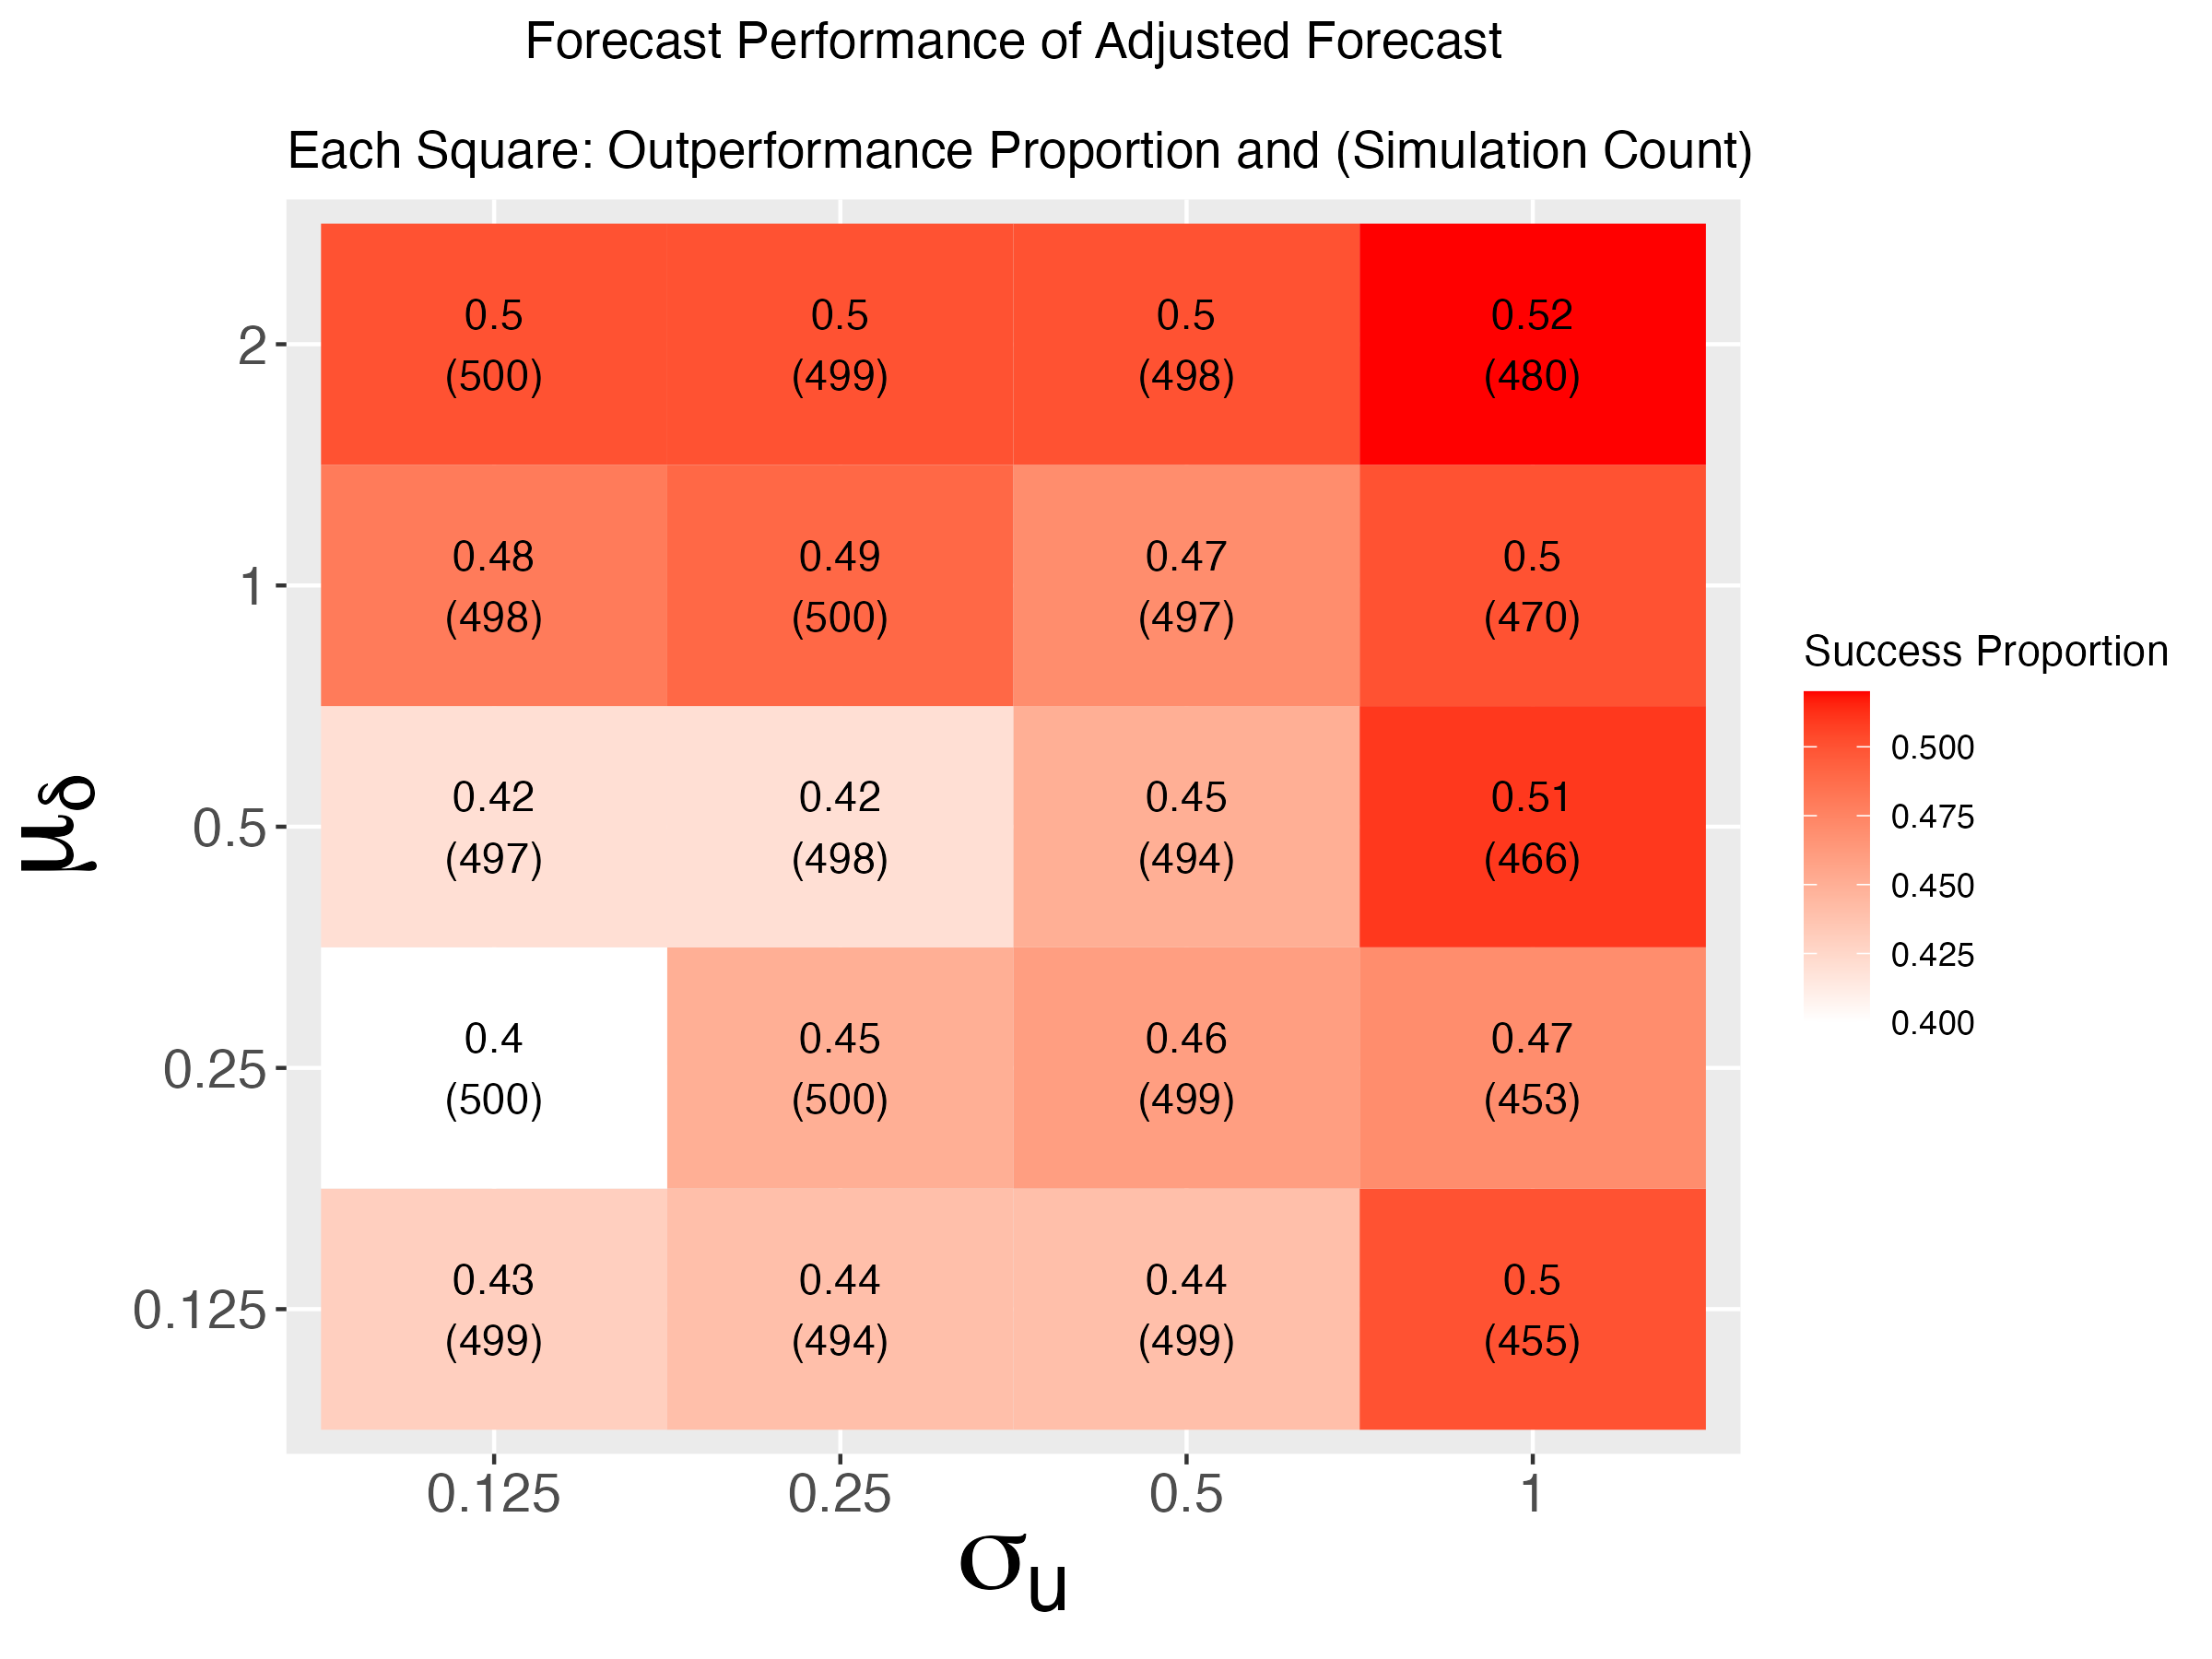
\includegraphics[scale = .42]{simulation_plots/Aug28_224311_2024_mu[delta]_sigma[u].png}
        \caption{Fixed values: $\mu_{v} = .125, \sigma_{v} = .125, \mu_{\omega^{*}} = .125$}\label{fig:sim_1}
    \end{subfigure}\hspace{12mm} %
    \begin{subfigure}{.44\linewidth} 
      \centering
        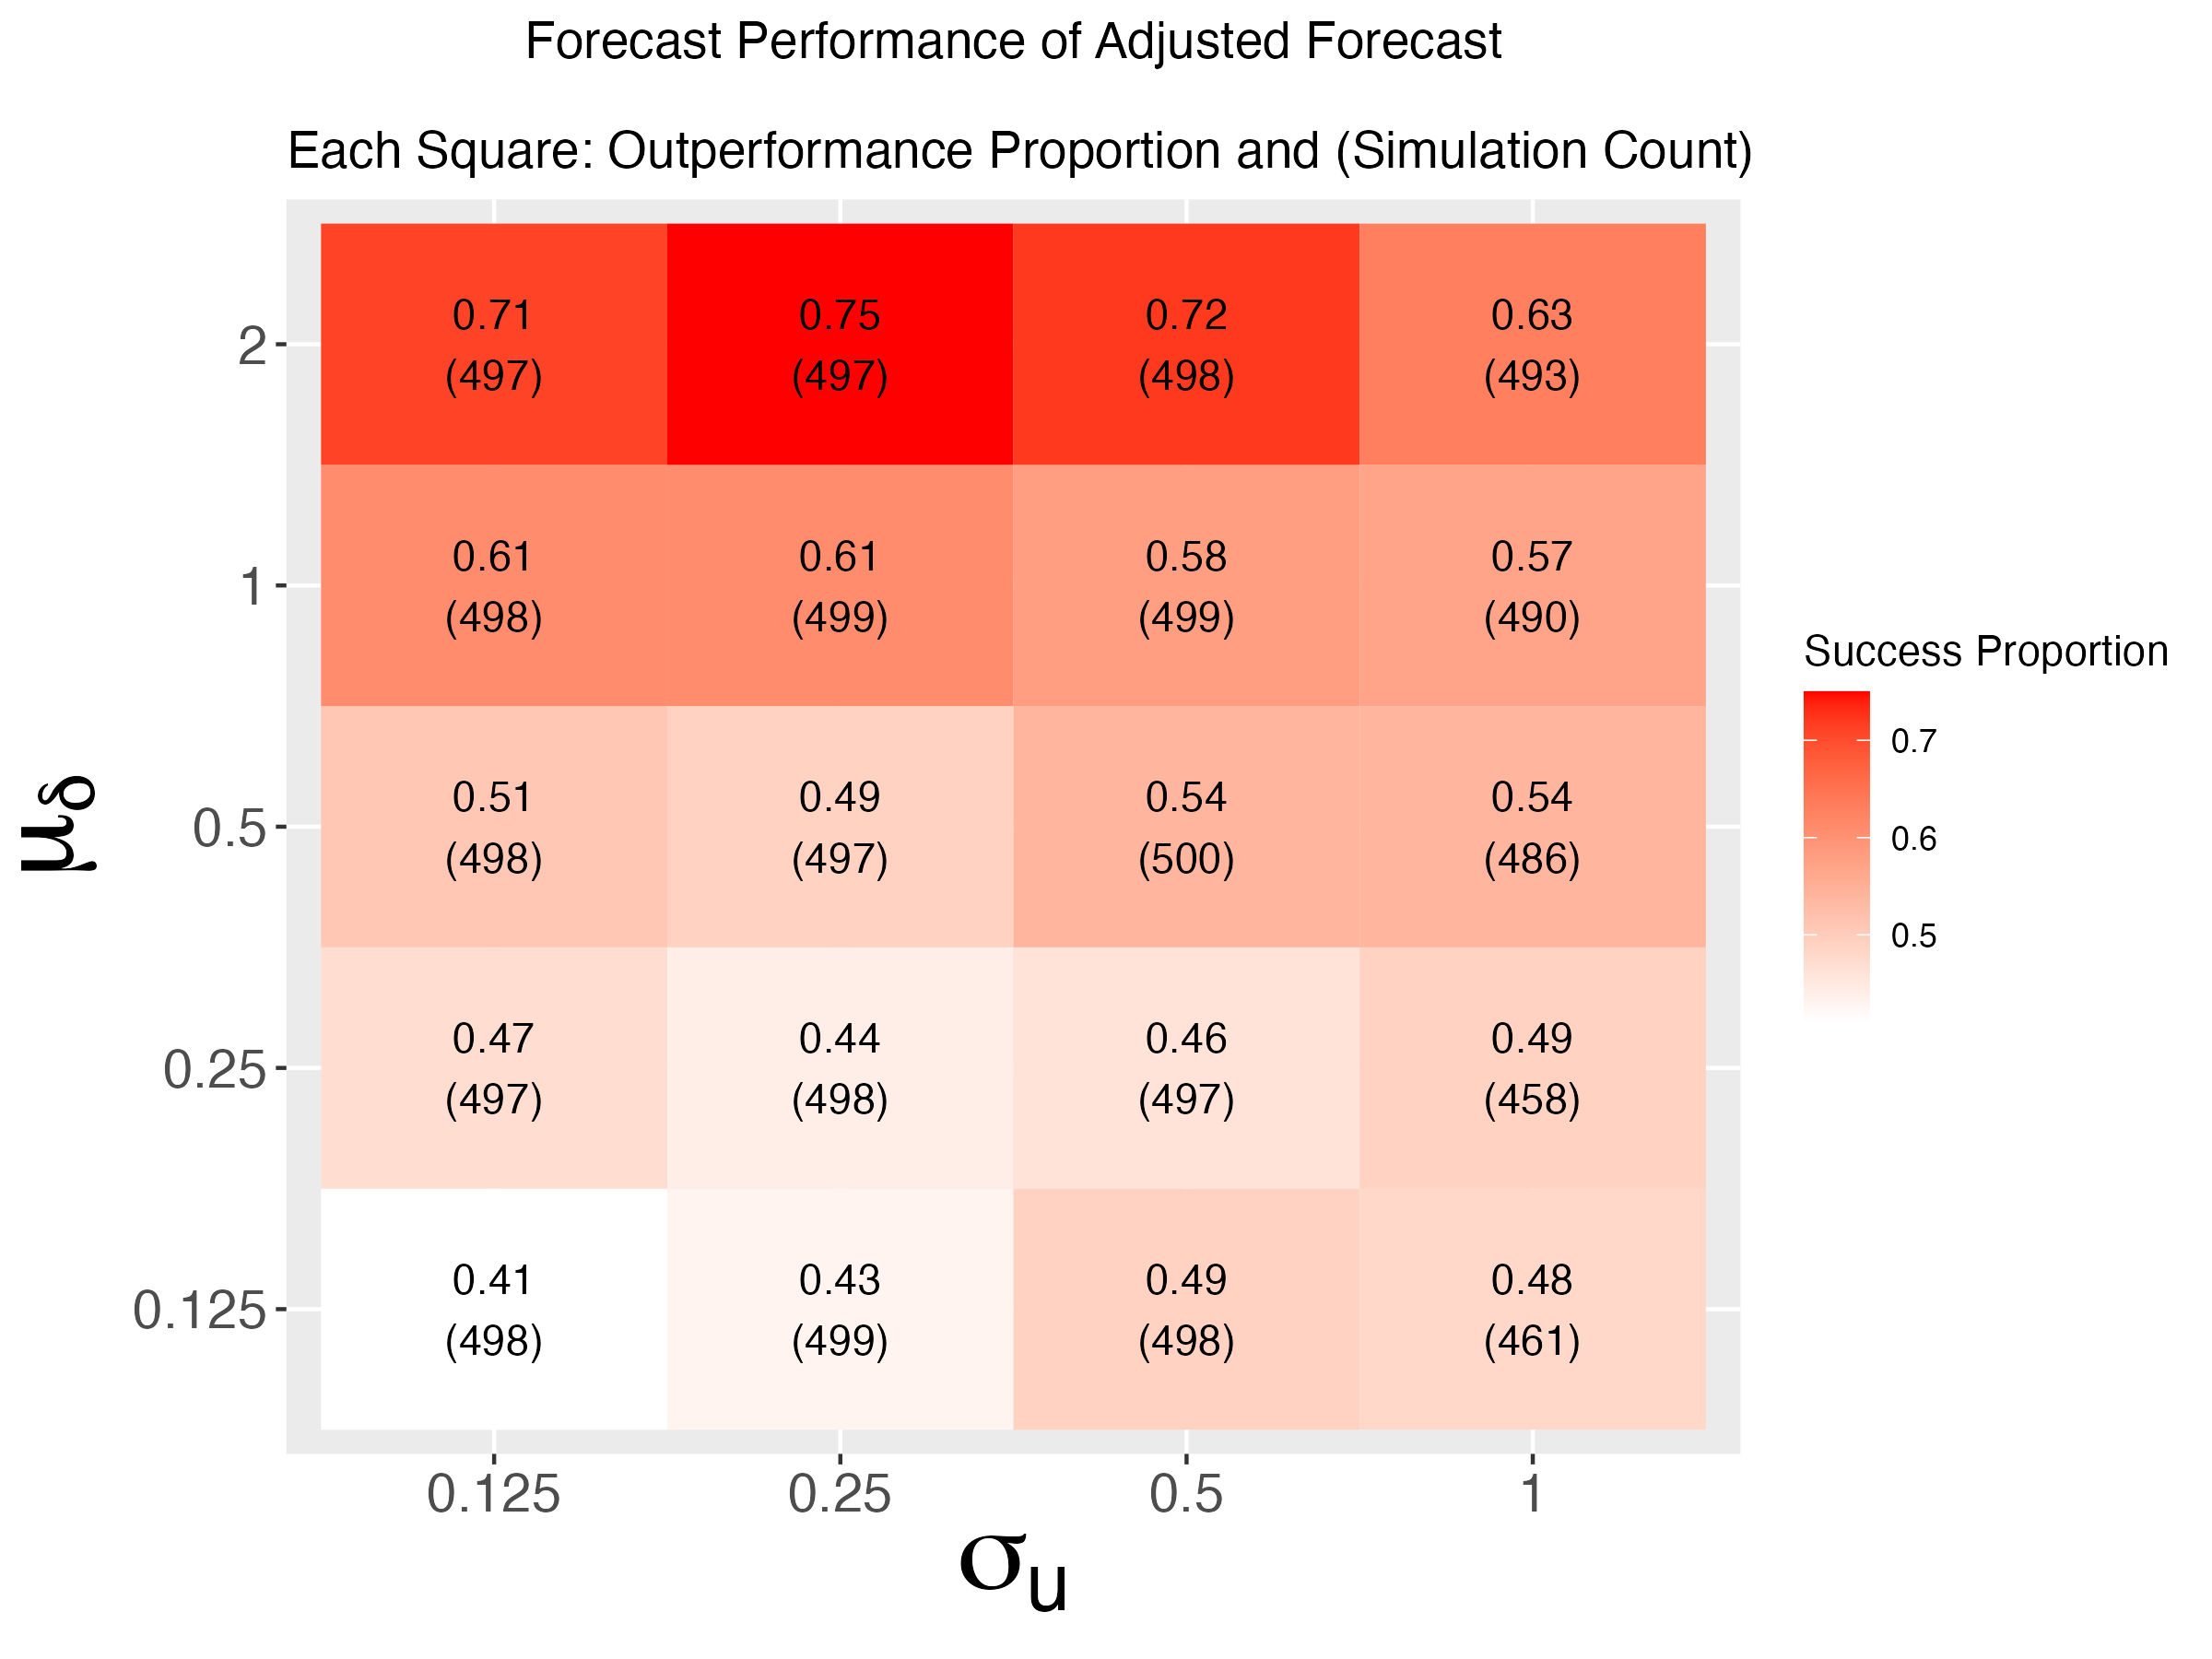
\includegraphics[scale=.42]{simulation_plots/Aug28_224317_2024_mu[delta]_sigma[u].png}
        \caption{Fixed values: $\mu_{v} = .5, \sigma_{v} = .125, \mu_{\omega^{*}} = .125$}\label{fig:sim_2}
    \end{subfigure}

    \begin{subfigure}{.44\linewidth} 
      \centering
        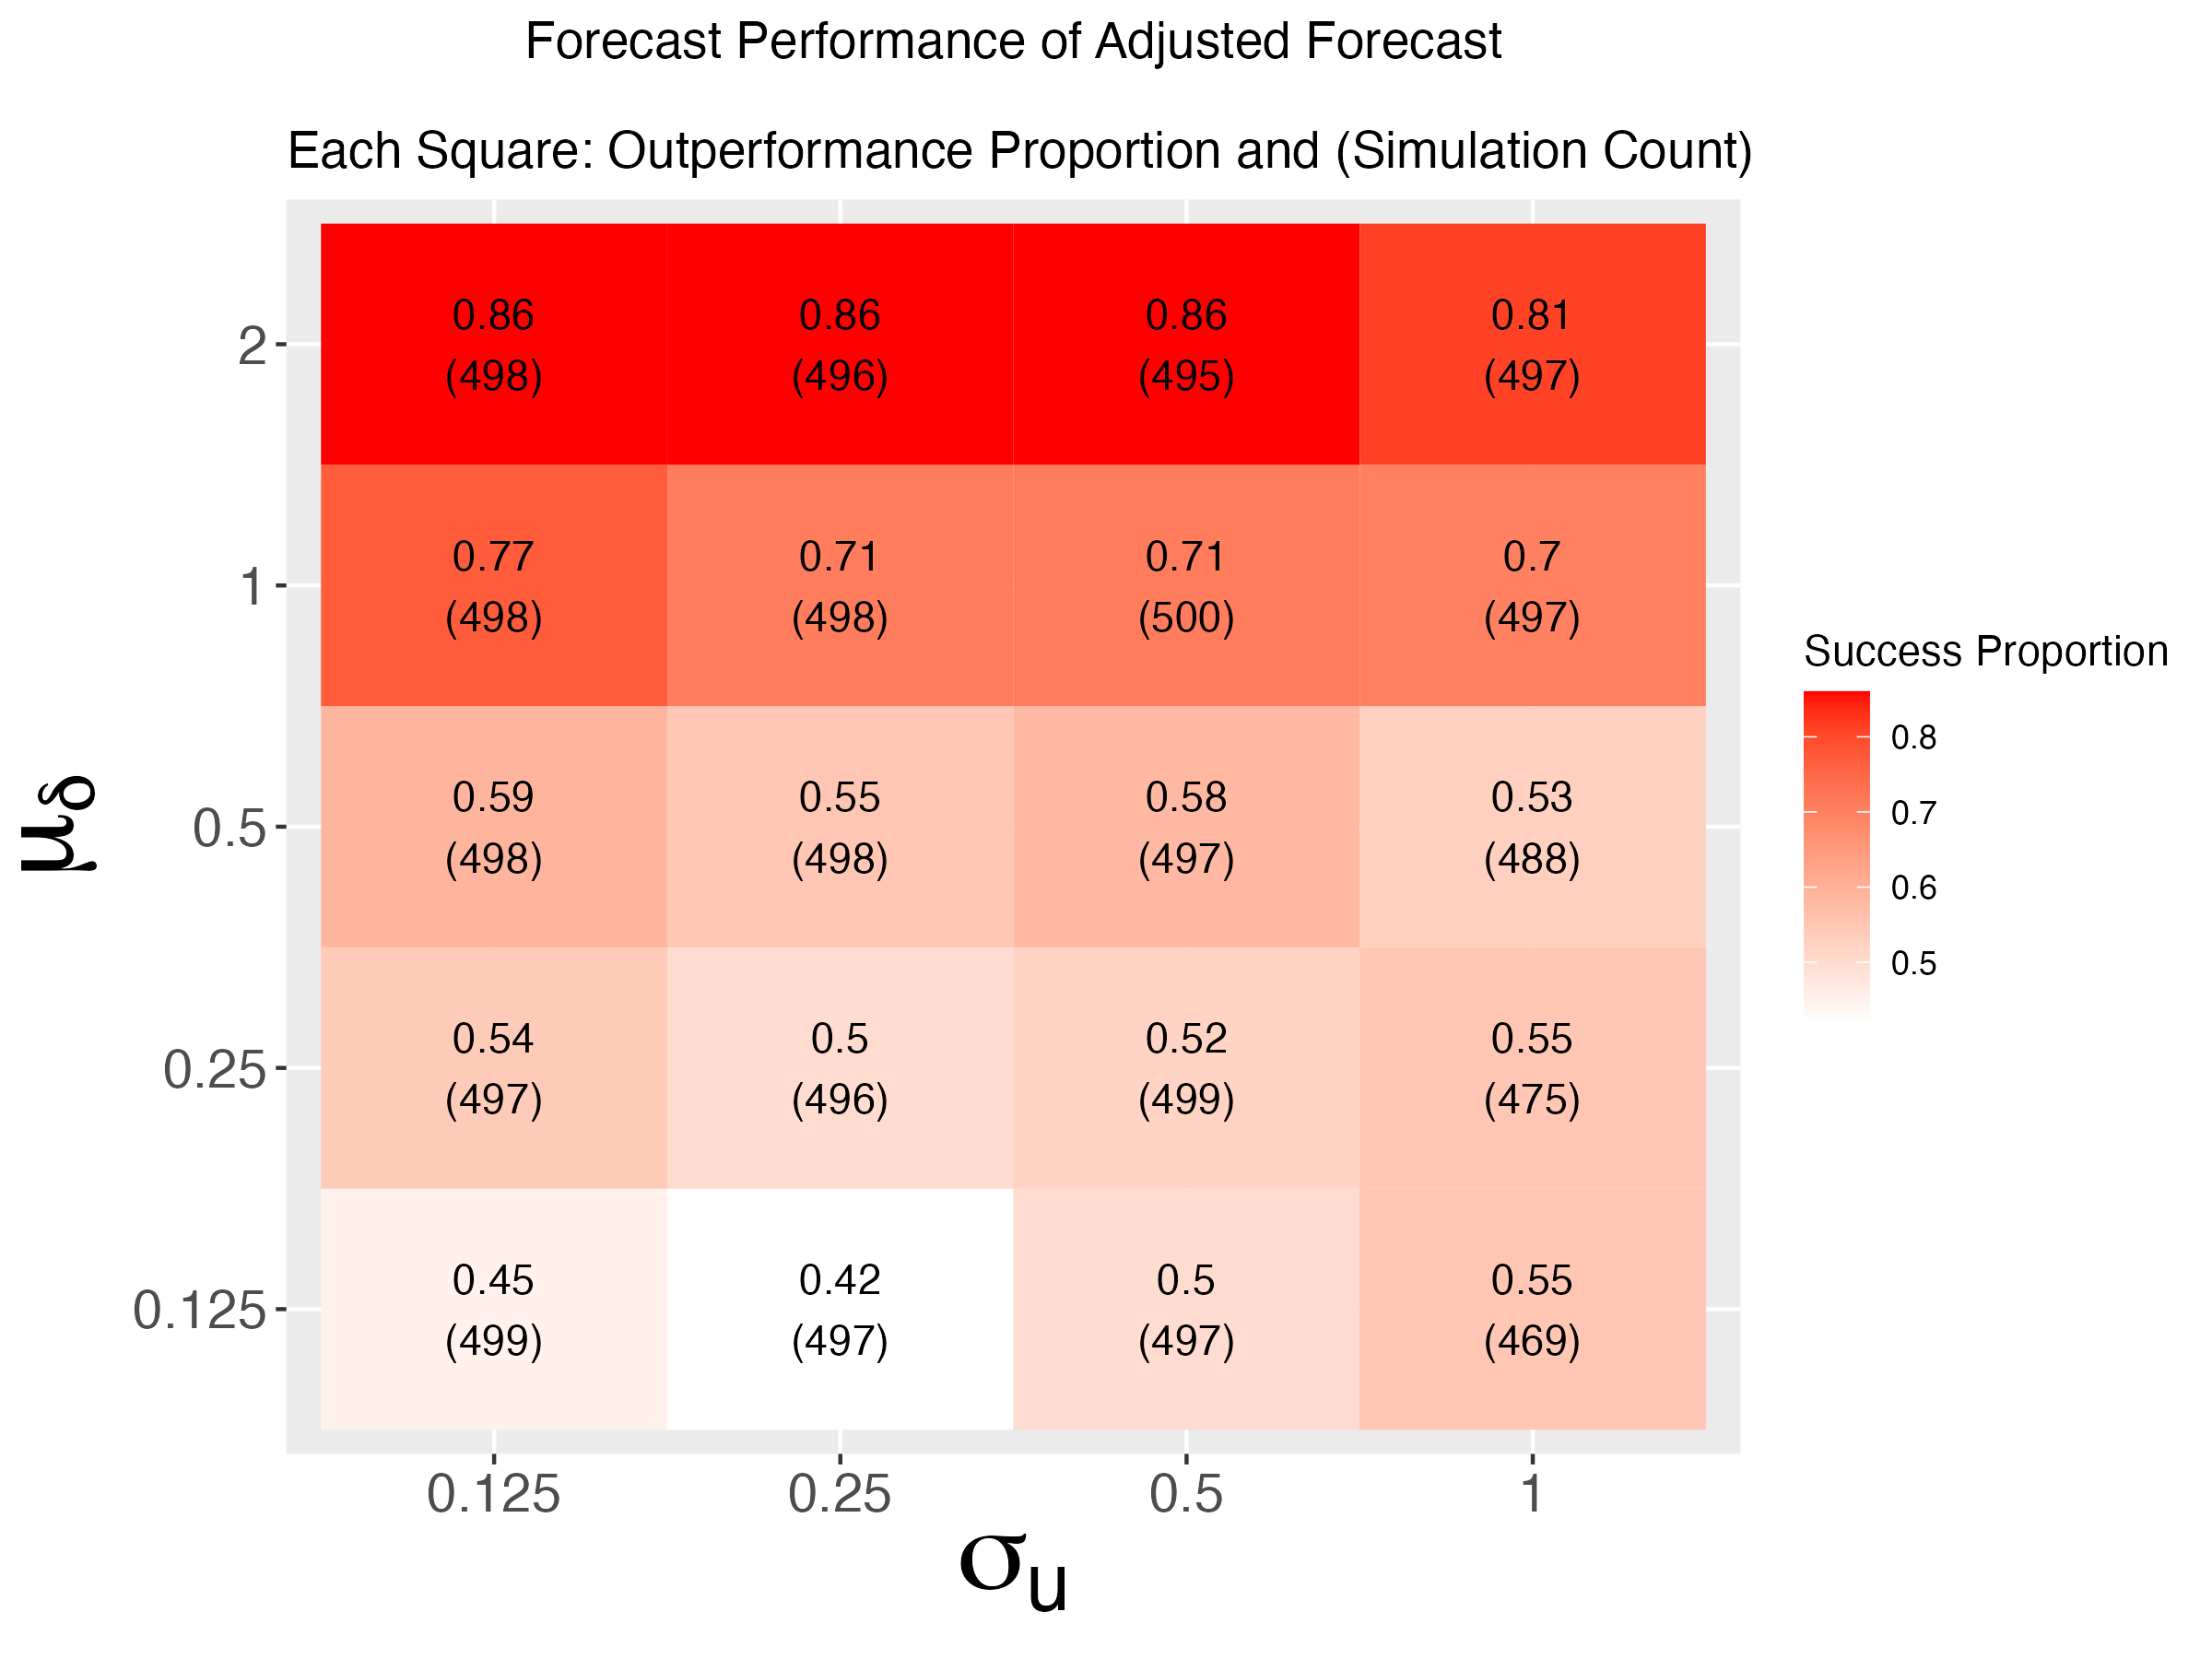
\includegraphics[scale=.42]{simulation_plots/Aug28_224322_2024_mu[delta]_sigma[u].png}
        \caption{Fixed values: $\mu_{v} = 1, \sigma_{v} = .125, \mu_{\omega^{*}} = .125$}\label{fig:sim_3}
    \end{subfigure}
    
        \caption{In the progression from \ref{fig:sim_1} to \ref{fig:sim_2} to \ref{fig:sim_3}, we see that increasing $\mu_{\delta}$ leads to improved performance of the adjusted forecast, and this effect is intensified as $\mu_{v}$ increases.  However, it is not consistently true that an increasing noise undermines the performance of the adjusted forecast.  Rather, that phenomenon requires both large quantites of $\mu_{\delta}$ and $\mu_{v}$.}
        \label{fig:signoise}
      \end{figure}

  \begin{figure}[!h]
    \centering
    \textbf{Interaction between Signal and Volatility Profile Means}\par\medskip
  \begin{subfigure}{.44\linewidth} 
    \centering
      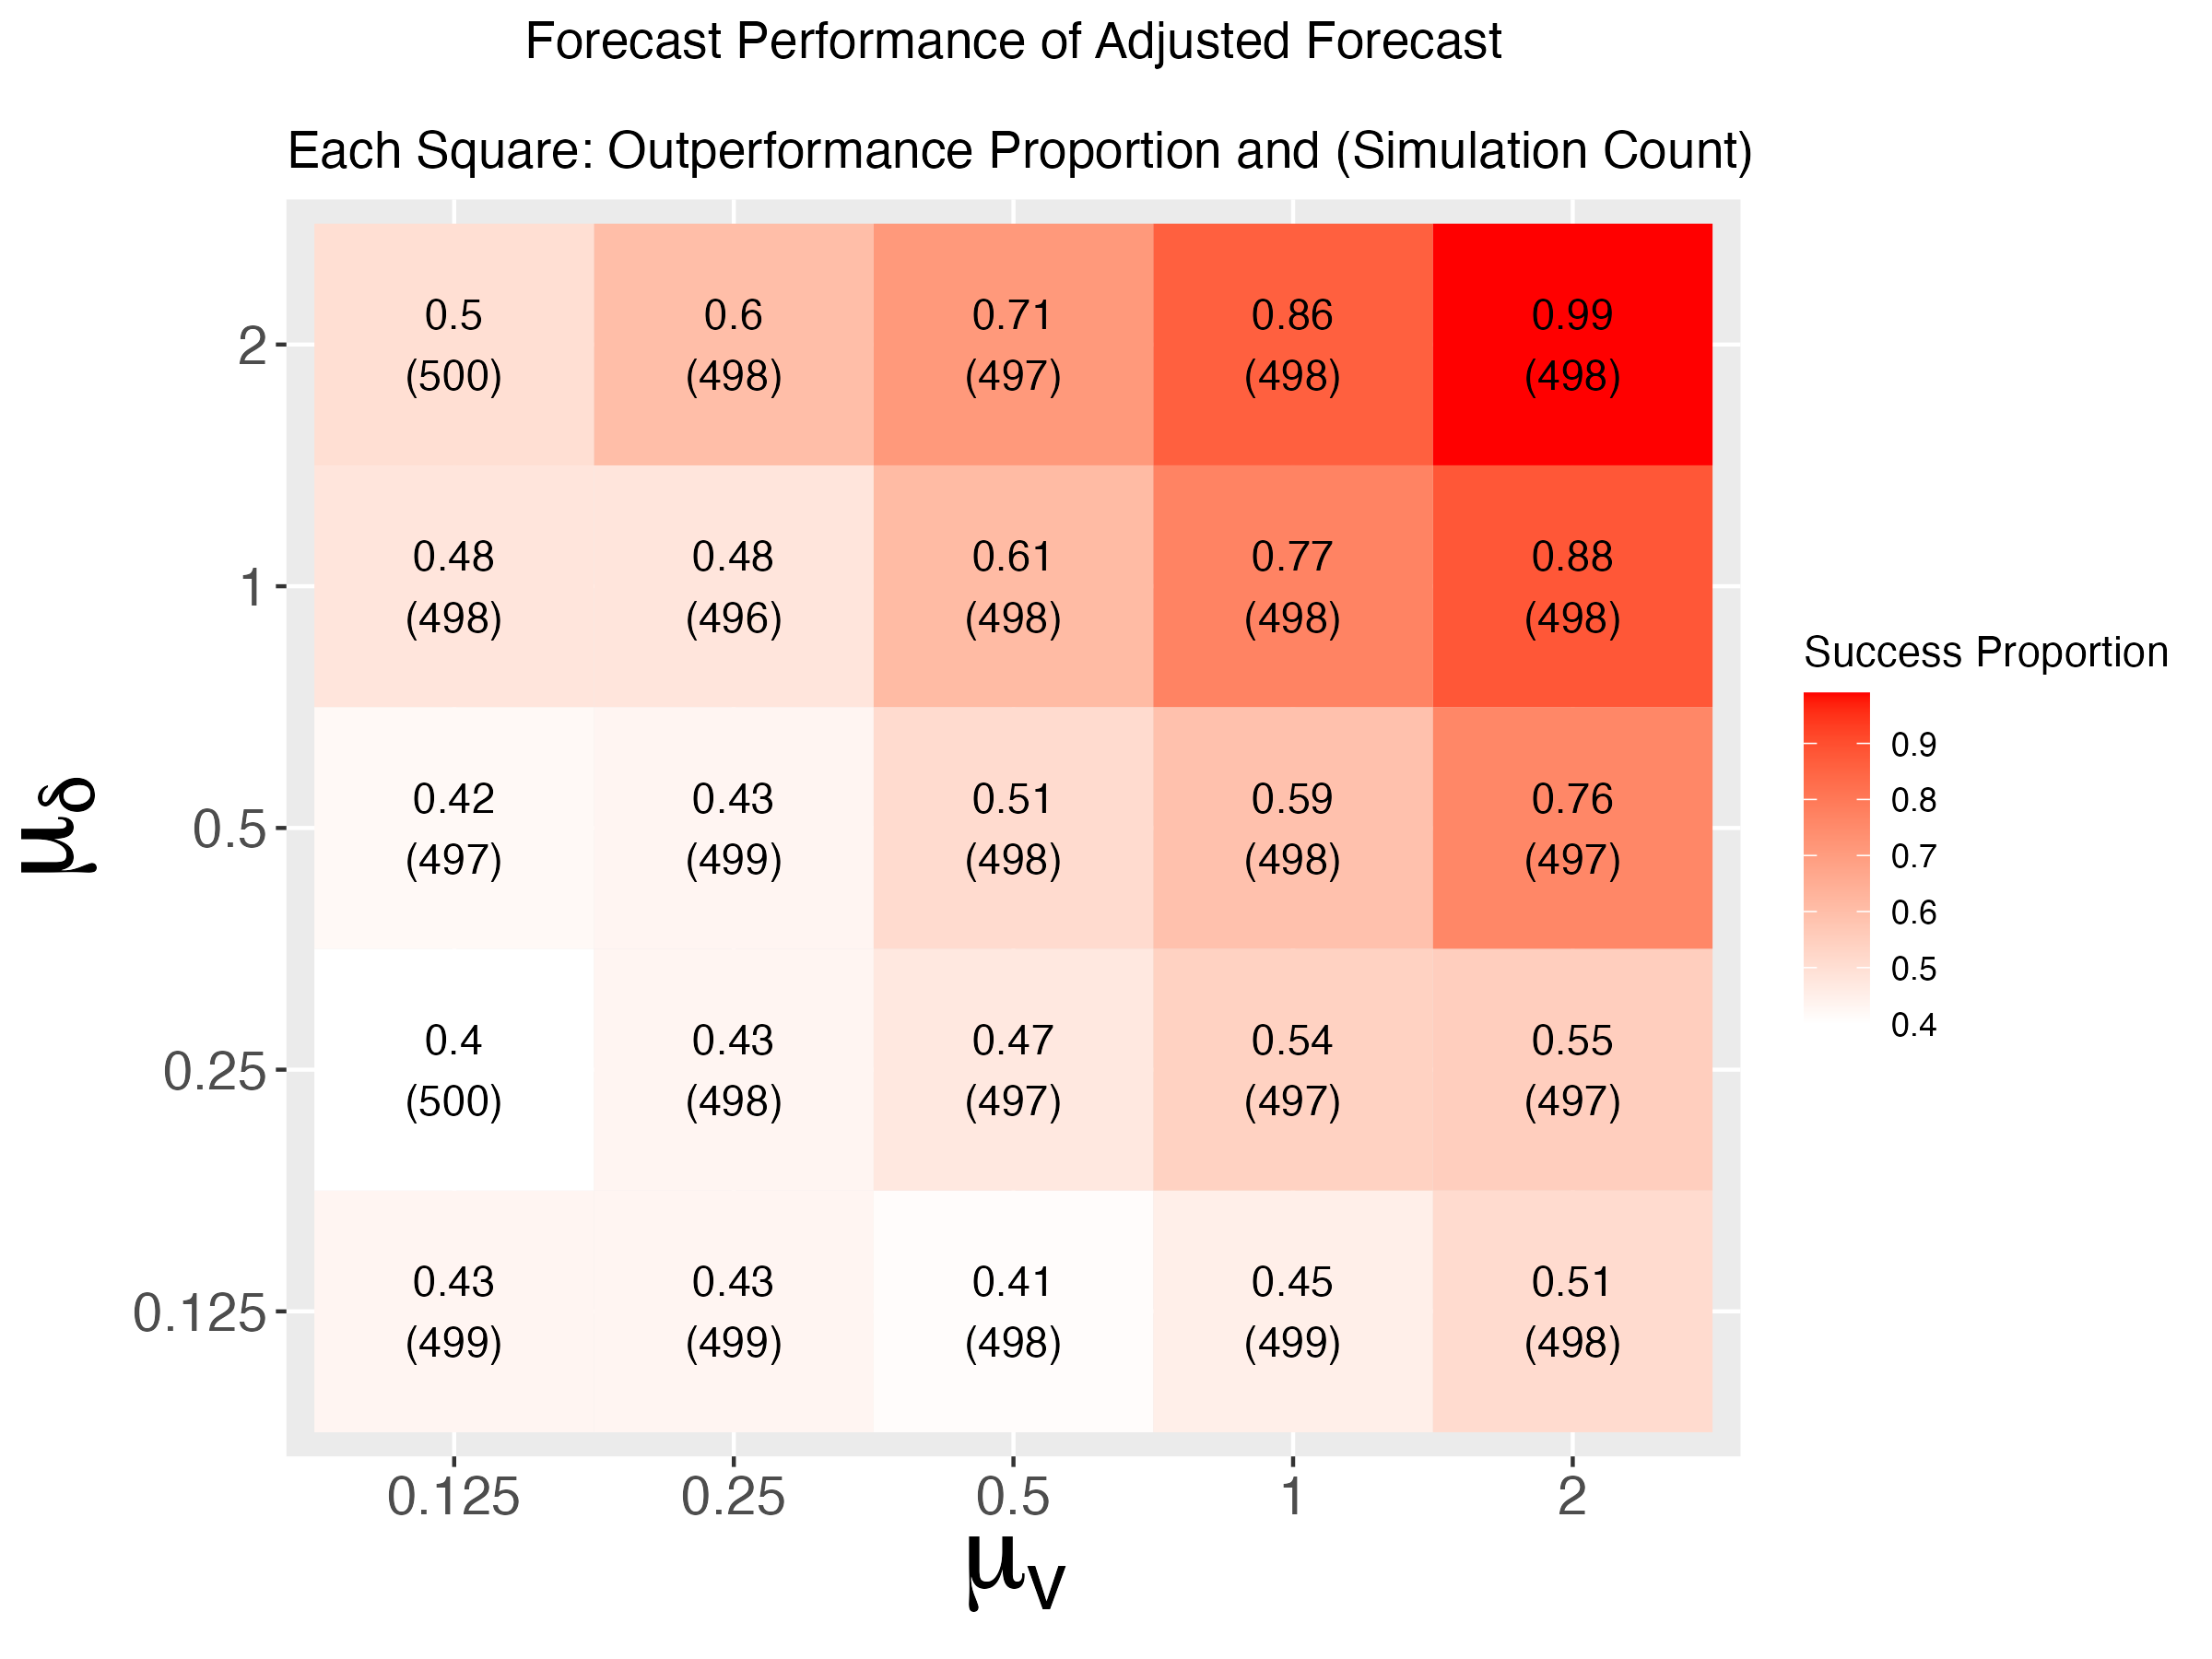
\includegraphics[scale = .42]{simulation_plots/Aug28_224330_2024_mu[delta]_mu[v].png}
      \caption{Fixed values: $\sigma_{v} = .125, \mu_{\omega^{*}} = .125, \sigma_{u} = .125$}\label{fig:sim_4}
  \end{subfigure}\hspace{12mm} %
  \begin{subfigure}{.44\linewidth} 
    \centering
      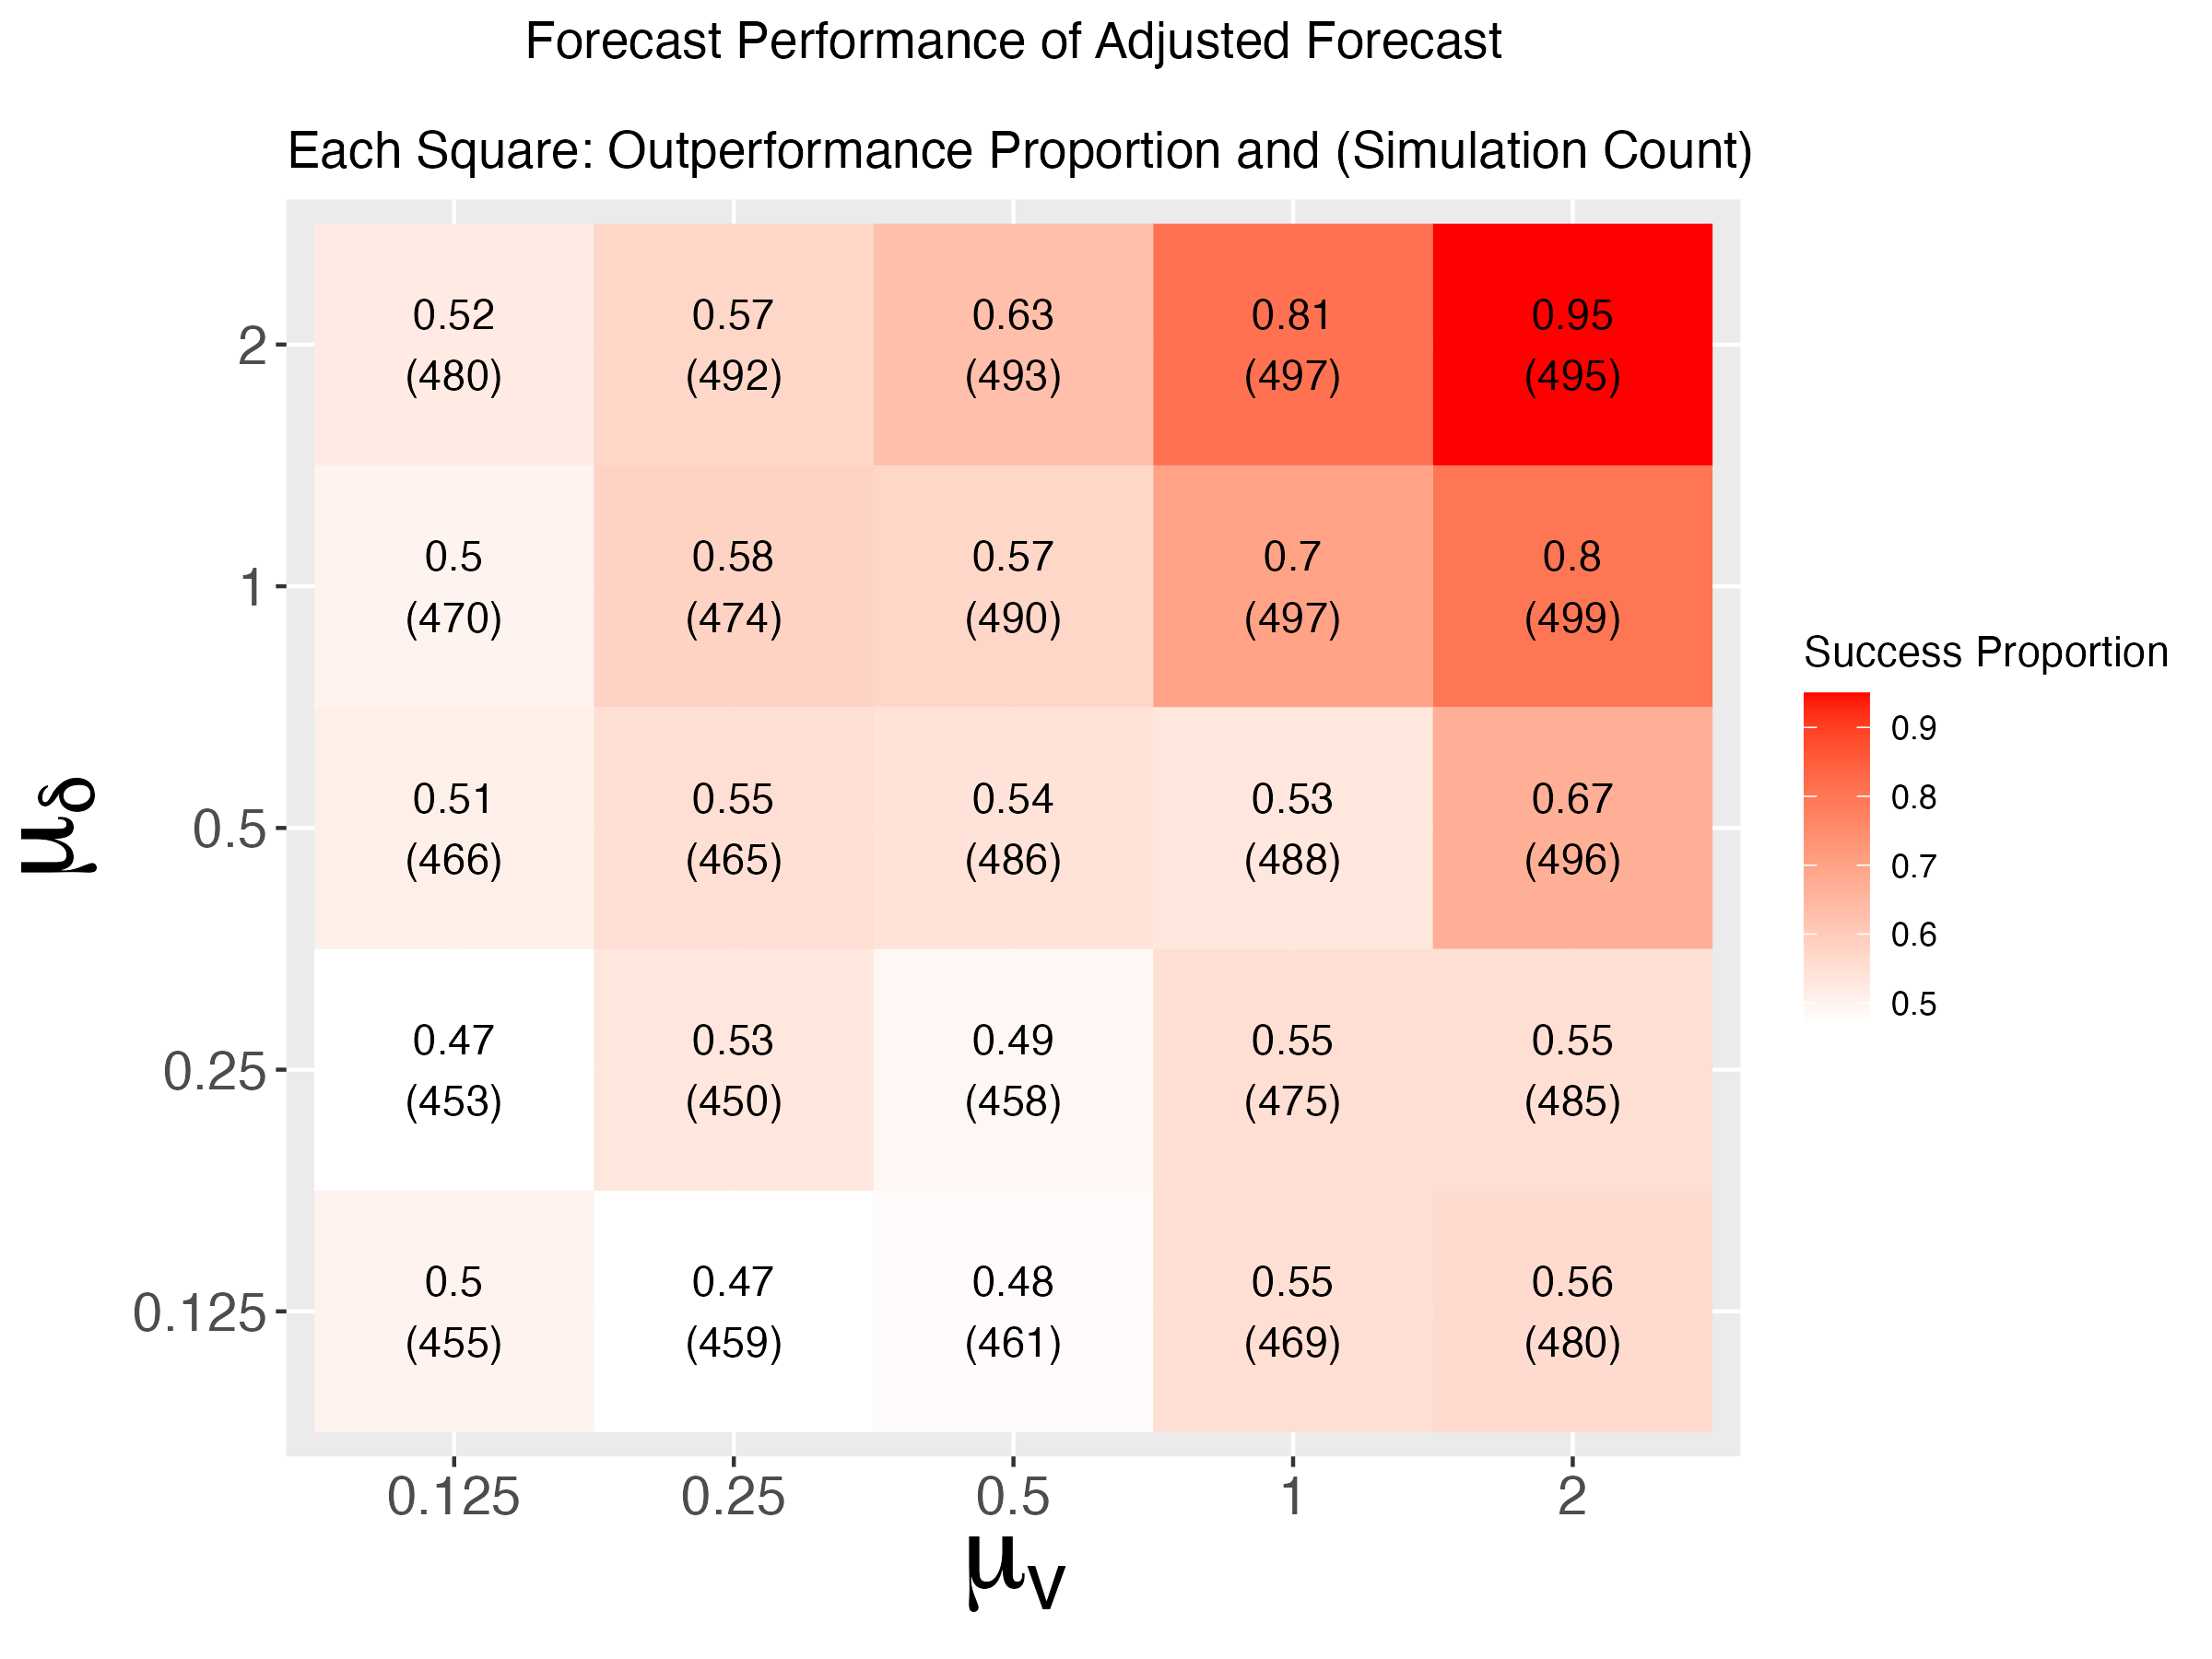
\includegraphics[scale=.42]{simulation_plots/Aug28_224337_2024_mu[delta]_mu[v].png}
      \caption{Fixed values: $\sigma_{v} = .125, \mu_{\omega^{*}} = .125, \sigma_{u} = 1$}\label{fig:sim_5}
  \end{subfigure}
  
      \caption{We compare the interaction of $\mu_{\delta}$ and $\mu_{v}$ at two different levels of shock noise.  In the low-noise regime, the peak performance of the adjusted forecast is higher, and the ascent is faster along both dimensions.   However, in the high-noise regime, the adjusted forecast performs well even at low levels of $\mu_{\delta}$ and $\mu_{v}$.}
      \label{fig:sig_volprof}
    \end{figure}

\begin{figure}[!h]
  \centering
  \textbf{Interaction between Shock Intercept and Shock Noise}\par\medskip
\begin{subfigure}{.44\linewidth} 
  \centering
    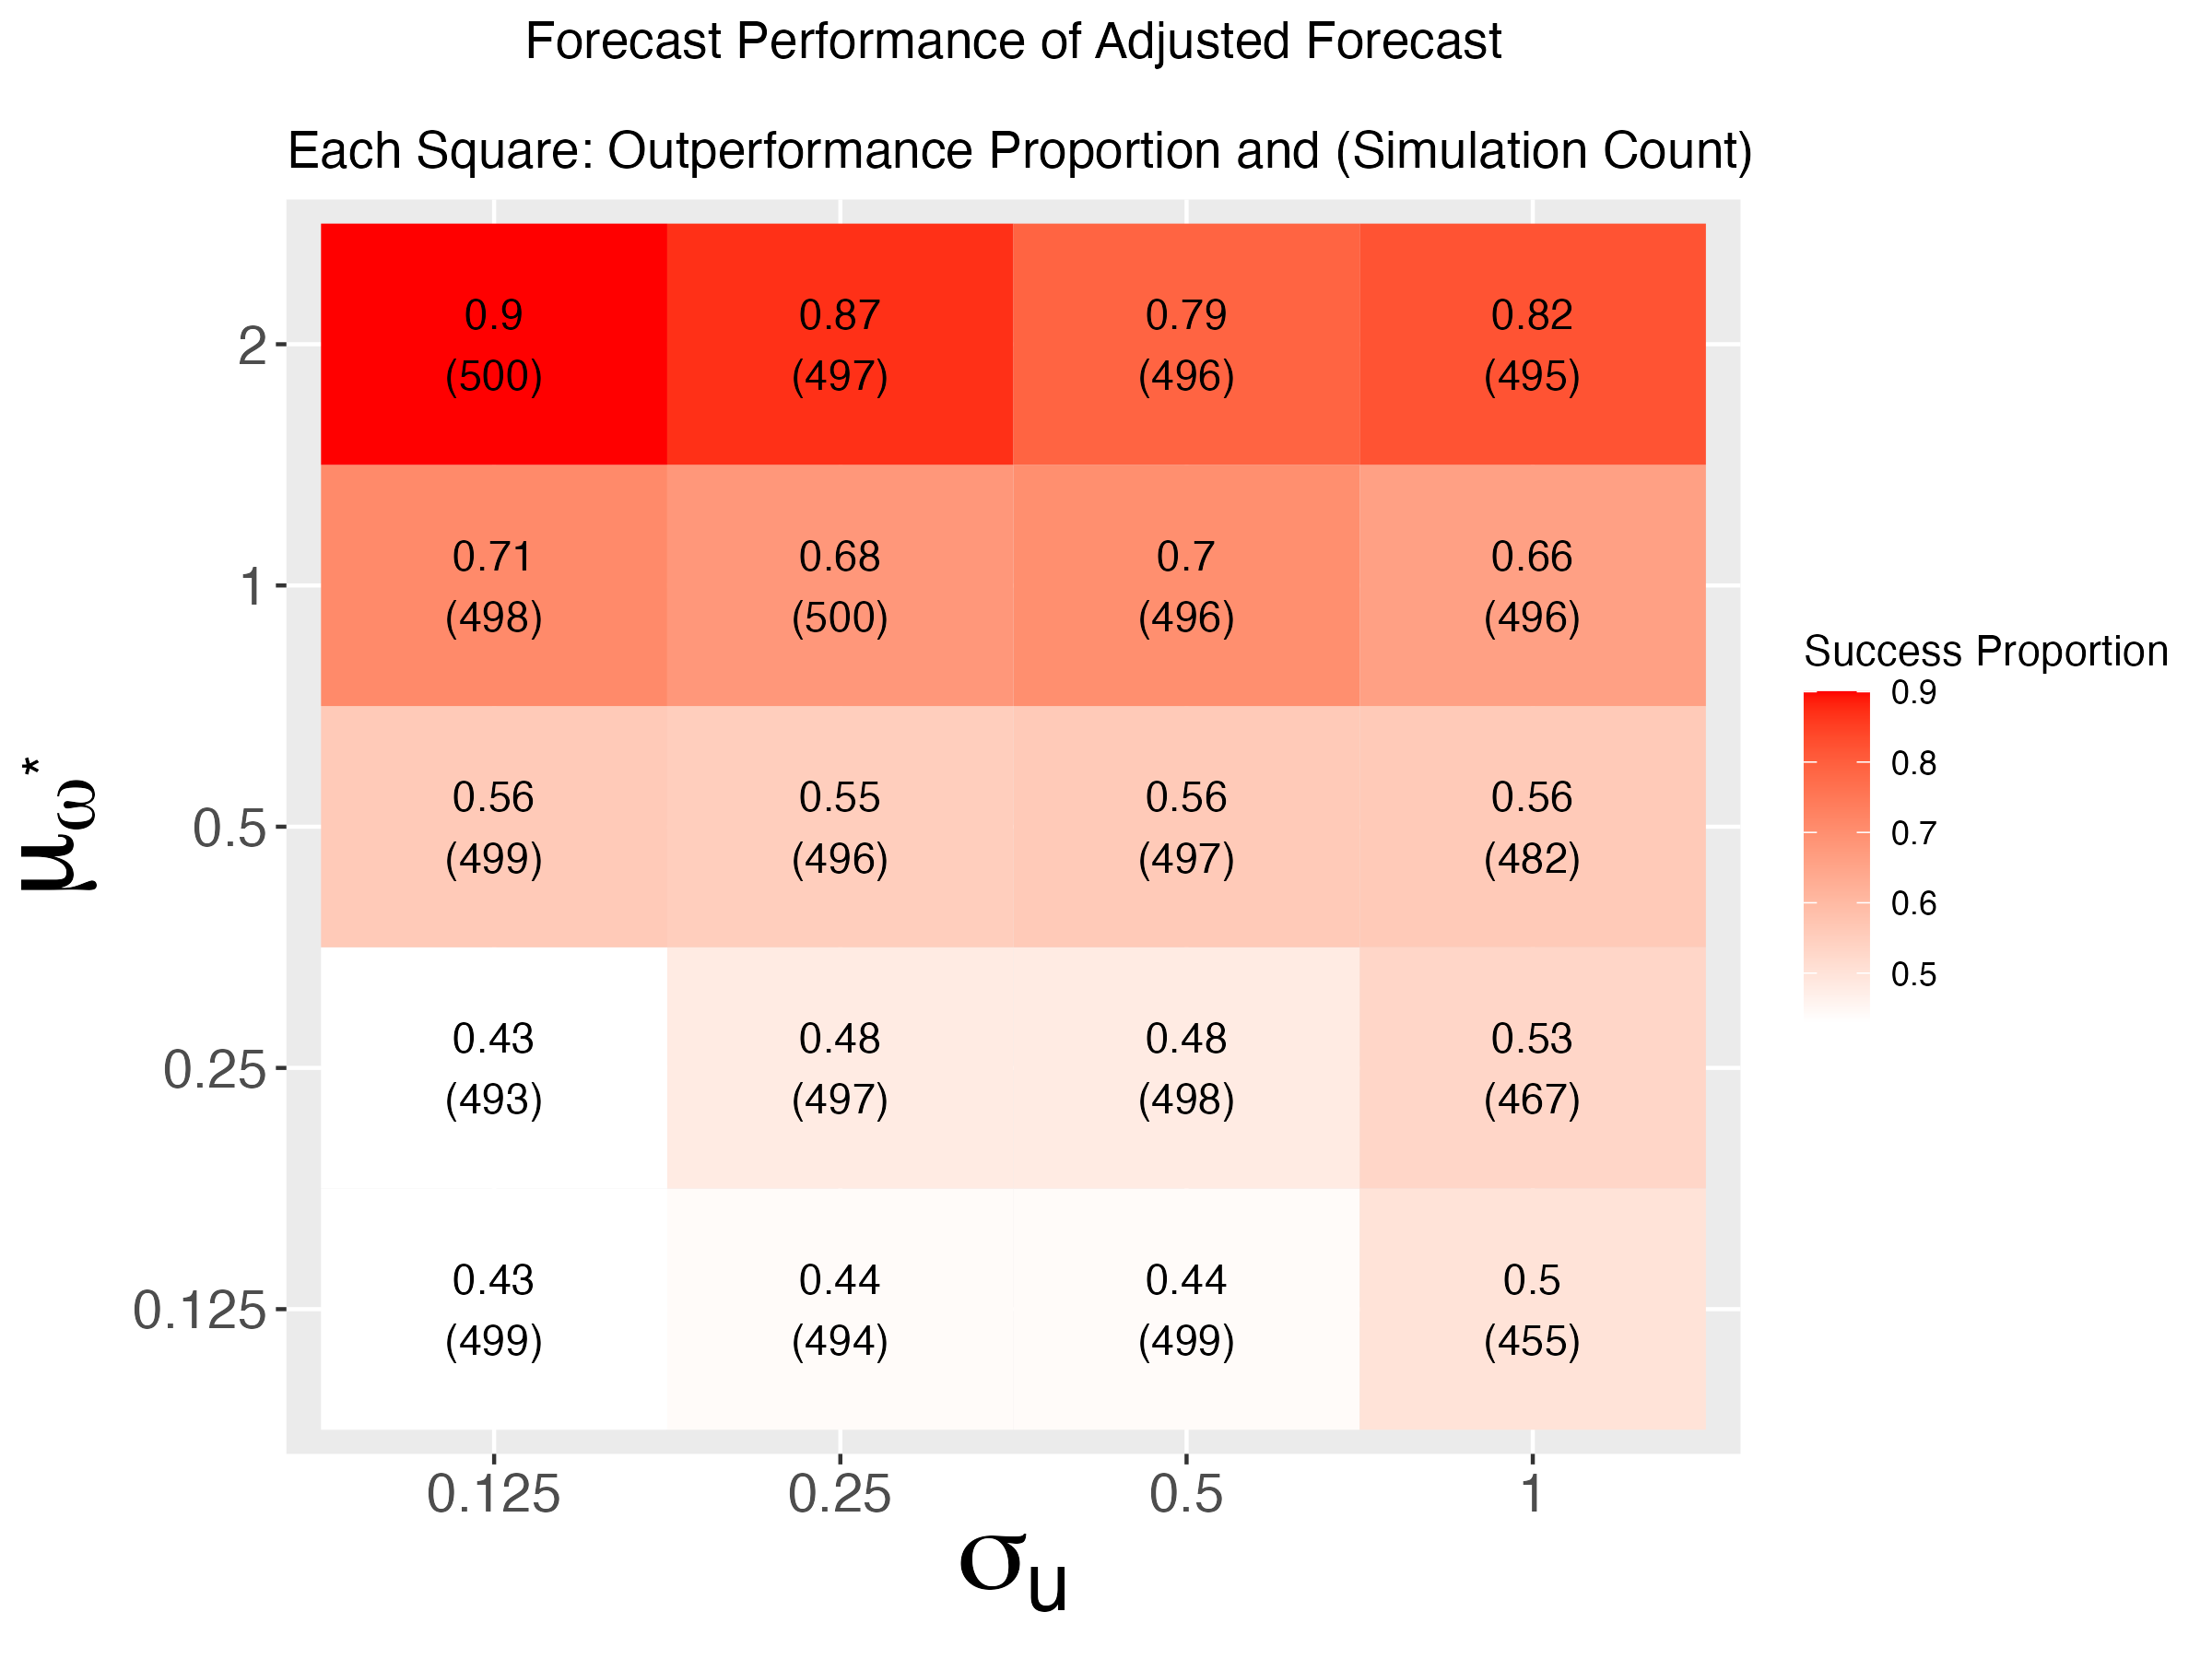
\includegraphics[scale = .42]{simulation_plots/Aug28_224451_2024_mu[omega^*]_sigma[u].png}
    \caption{Fixed values: $\mu_{v} = .125, \sigma_{v} = .125, \delta = .125$}\label{fig:sim_6}
\end{subfigure}\hspace{12mm} %
\begin{subfigure}{.44\linewidth} 
  \centering
    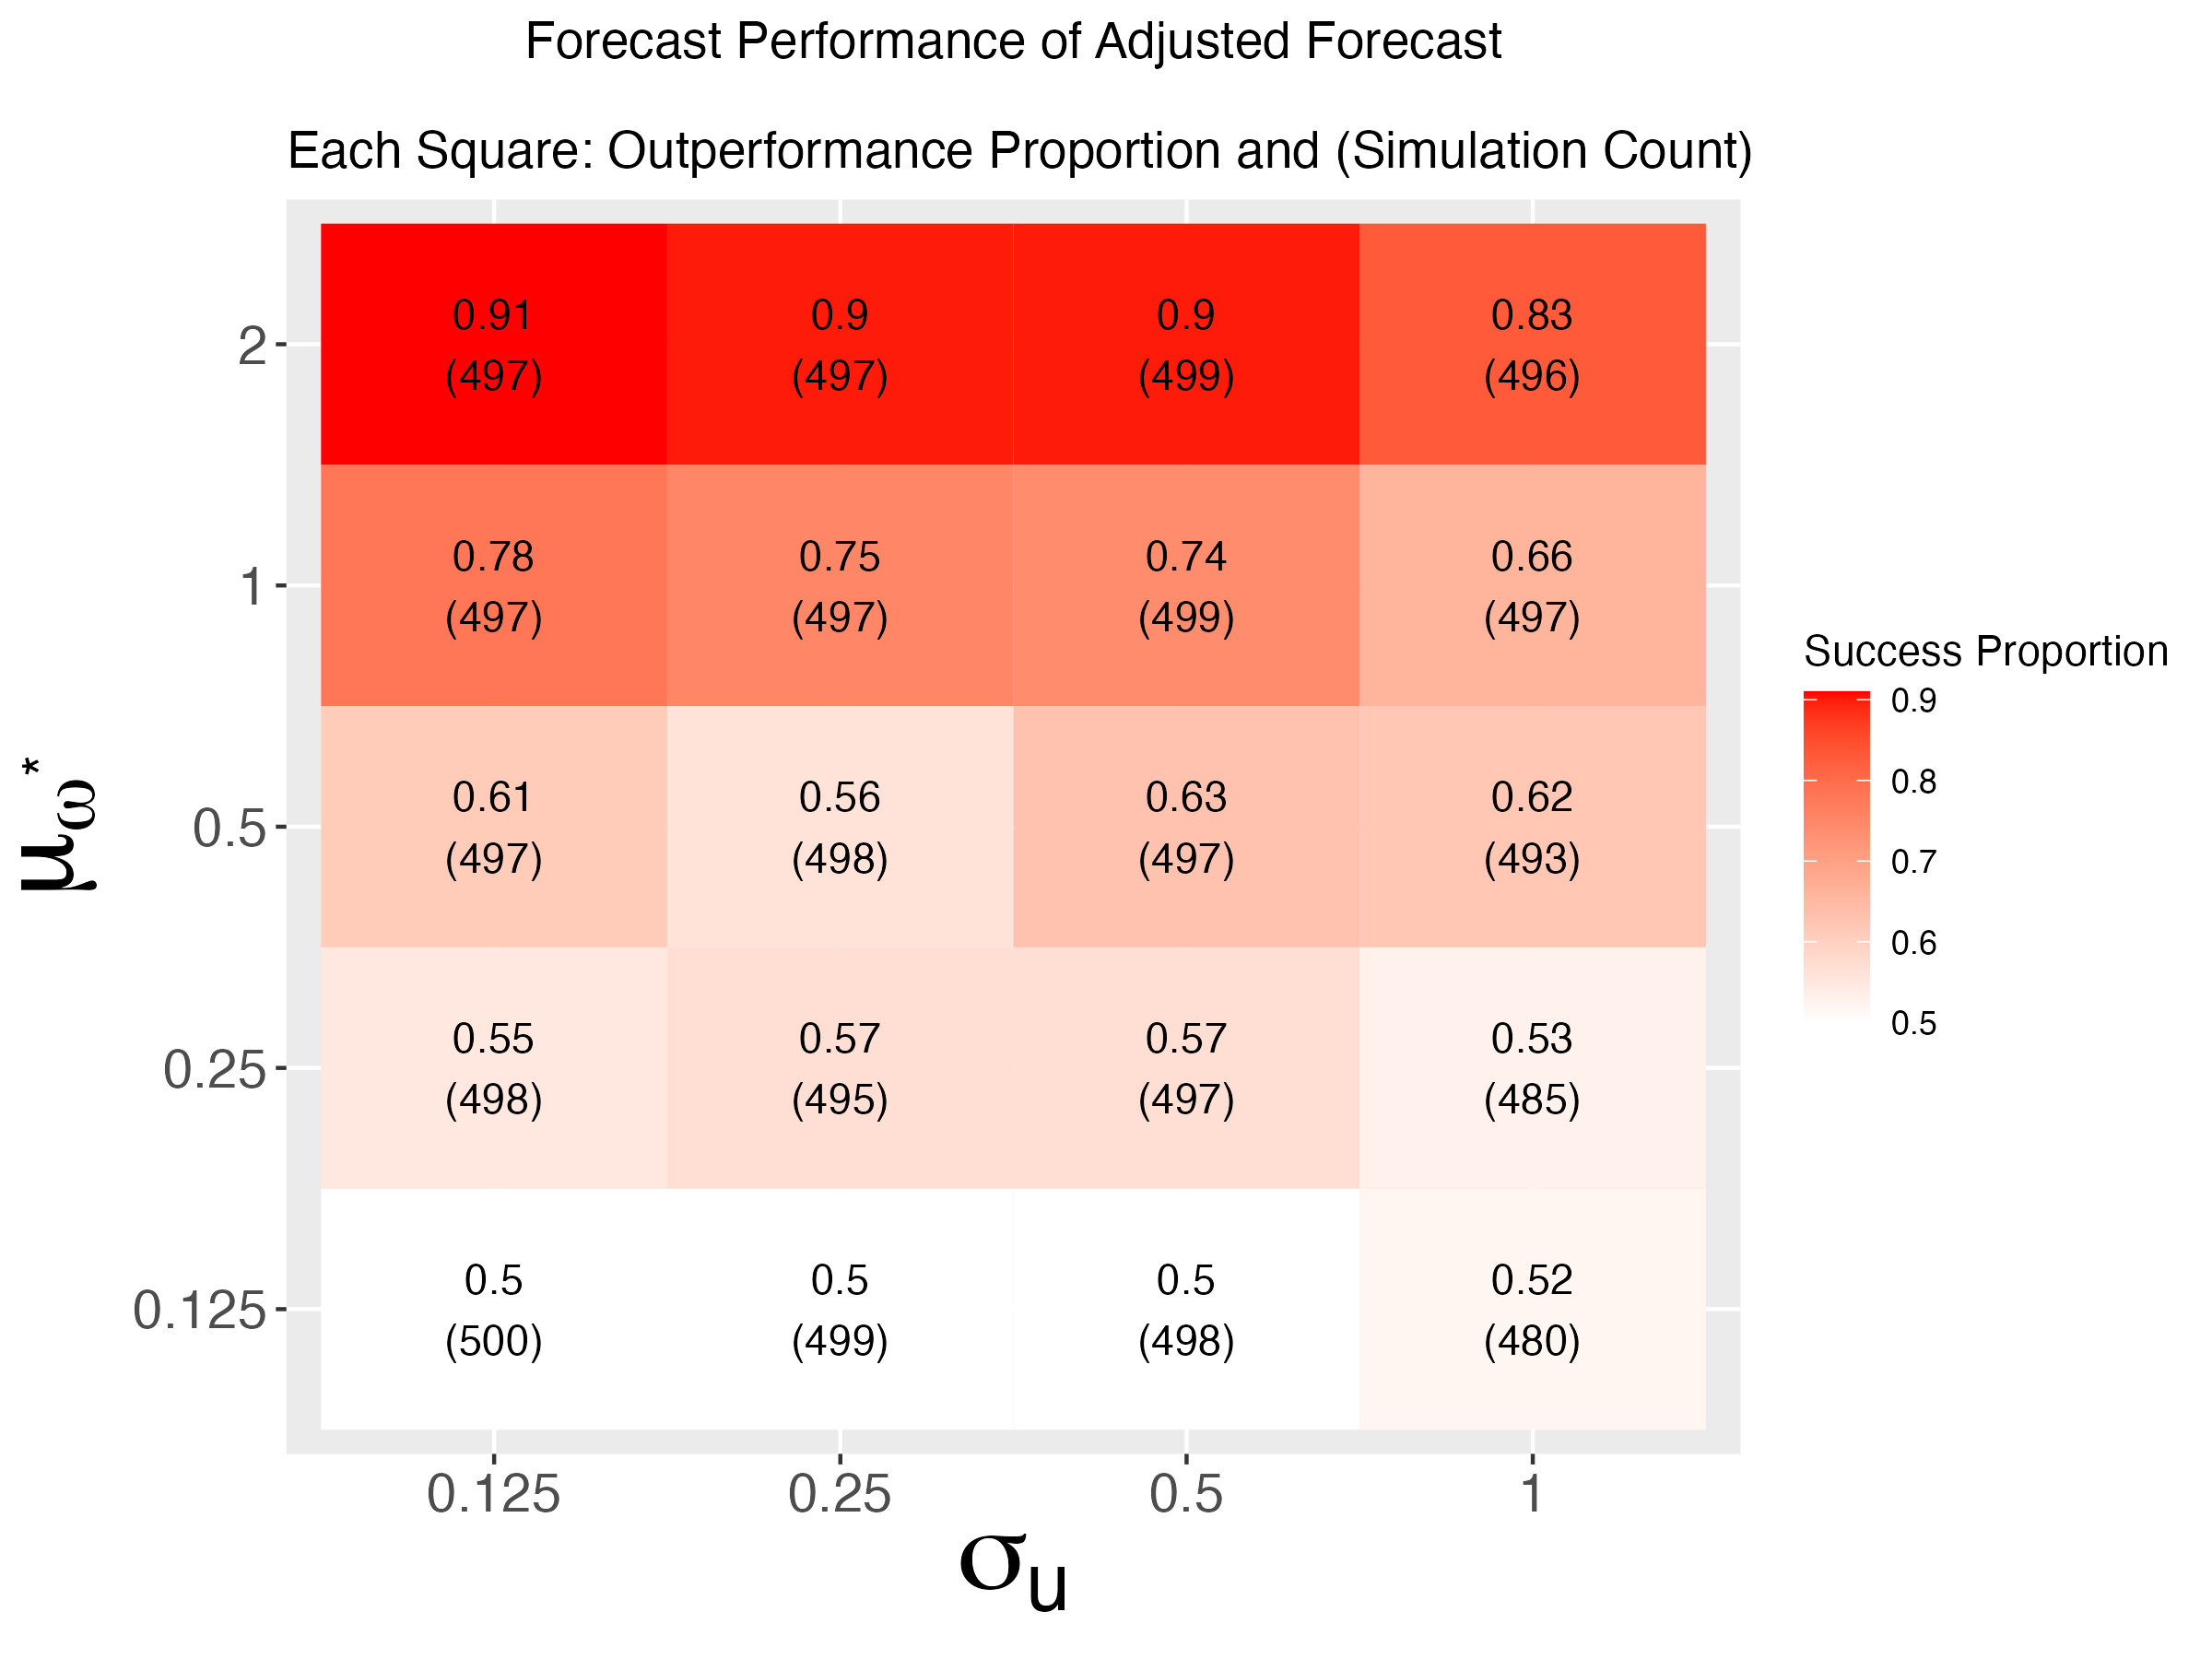
\includegraphics[scale=.42]{simulation_plots/Aug28_224455_2024_mu[omega^*]_sigma[u].png}
    \caption{Fixed values: $\mu_{v} = .125, \sigma_{v} = .125, \delta = 2$}\label{fig:sim_7}
\end{subfigure}

    \caption{The interaction between the intercept $\mu_{\omega^{*}}$ and $\sigma_{u}$ suggests that the parameters behave as expected.  However, a larger value of $\delta$ in \ref{fig:sim_7} attenuates the effect of increasing noise.}
    \label{fig:intercept_noise}
  \end{figure}

\clearpage 

\section{Forecasting after the results of the 2016 US presidential election}\label{Real Data Example}

We demonstrate the applicability of our methodology using a real data set at the intersection of financial trading and electoral politics. The goal of this analysis will be to provide a forecast for the volatility of IYG\footnote{It has been noted that GARCH effects are more attenuated in aggregated returns \citep{zivot2009practical}, which suggests against using the S\&P 500 or similar indices as an example.} (an ETF composed of American financial majors JPMorgan, Bank of America, etcetera) on Wednesday November 9th, 2016 using only the information available at the close of US financial markets at 4pm ET on November 8th, 2016, either after Donald Trump won the 2016 US presidential election or in a scenario in which Trump would win the day. Our specifications for this analysis are outlined below:

%In the spring of 2016 in the United States, the Republican Party's primary election process narrowed down candidates until Donald J. Trump cleared the threshold of votes to win the nomination formally at the party's convention that summer.  He would go on to face the Democratic Party's nominee, Hillary Rodham Clinton.   

%meets the standard of an interesting and notable event for which a quantitative researcher might seek a volatility point prediction.  On a more technical level, the election outcome was not known until the evening of election day, well after the closing of financial markets at 4pm Eastern Time.  This satisfies the condition that the shock be not yet digested by liquid markets.  We therefore proceed to make the following technical specifications in order to 


%From an ex-ante perspective, several qualities of the 2016 US election cycle as well as the candidates themselves made the election difficult to prognosticate.  The Electoral College permits victory without a majority or even plurality of the popular vote, which can render presidential races more competitive than a raw vote total would, elevating the uncertainty surrounding the country's future leadership.  The election featured no incumbent, ruling out any incumbent-advantage of the empirical, ``statistical" kind distinguished by \citet{mayhew2008incumbency}.  The Republican Party candidate espoused unorthodox, populist positions on matters such as healthcare, trade, and foreign policy, some of which could be considered rare in either of the major two parties.  Additionally, Donald J. Trump, lacking any experience in government --- either electoral or appointed service --- possessed neither a voting record nor any on-the-job performance for voters to judge or his opponents to attack. As one financial industry professional commented, comparing the 2016 election to the upcoming 2024 election, ``this time the markets will be aware of both possibilities and price them to some extent — we wouldn’t expect the same volatility as we saw in 2016 after the election" \citep{News_2024}. Gleaning signals from financial options markets and betting markets, \citet{wolfers2016financial} predicted that markets would decline prodigiously following a Trump victory in November 2016.  Finally, the election outcome delivered significant ``news", in the econometric sense of the word, in the simple sense that it was not predicted.  \citet{goodell2013us} found support for the theory that the polling-implied probabilities of election outcomes encode information about future macroeconomic conditions, which is itself reflected in market volatility.  In its final post before the election result, acclaimed forecasting outfit 538, headed by economist Nate Silver, predicted a Clinton victory with a probability of .714, more than 2-to-1 odds \citep{Silver_2016}, suggesting that Trump's victory was at least somewhat surprising.  The lack of uncertainty exerts downward pressure on volatility \citep{li2006presidential,bowes2018stock}, setting the table for a surprise.

%For all of these reasons and more, the aftermath of the 2016 presidential election meets the standard of an interesting and notable event for which a quantitative researcher might seek a volatility point prediction.  On a more technical level, the election outcome was not known until the evening of election day, well after the closing of financial markets at 4pm Eastern Time.  This satisfies the condition that the shock be not yet digested by liquid markets.  We therefore proceed to make the following technical specifications in order to predict the volatility of financial services ETF IYG\footnote{It has been noted that GARCH effects are more attenuated in aggregated returns \citep{zivot2009practical}, which suggests against using the S\&P 500 or similar indices as an example.} (an ETF composed of American financial majors JPMorgan, Bank of American, etcetera) on Wednesday November 9th, 2016.

\begin{enumerate}
    \item \textbf{Model choice} We assume a GARCH(1,1) for the daily log return series of IYG in each donor.  As argued in \citet{hansen2005forecast}, a GARCH(1,1) is rarely dominated by more heavily-parameterized GARCH specifications.  It thus provides a defensible choice when motivation or time for choosing another model is lacking.  For the time series under study and the donor series alike, we fit a GARCH(1,1) on almost four years of market data prior to the shock.

    \item \textbf{Covariate Choice} We choose covariates that could plausibly satisfy the model assumptions spelled out earlier, that is, risk-related and macroeconomic covariates that could plausibly be weighted and summed in a shock distribution.  We thus choose the log return Crude Oil (CL=F), the VIX (VIX) and the log return of the VIX, the log returns of the three-month, five-year, ten-year, and thirty-year US Treasuries.  Finally, we include the squares of the demeaned log return of IYG for the three trading days preceding the shocks, in an effort to capture the `local' ARCH effects prior to the shocks.  For each variable in the volatility profile, we compute the sample mean and sample standard deviation across the $n+1$ events, allowing us to scale the variables to have zero mean and unit variance.  Hence, no single variable can dominate the distance-based weighting procedure.

    \item \textbf{Donor pool construction} We choose the three most recent US presidential elections prior to the 2016 election as well as several Brexit-related events in the first half of 2016.  The inclusion of the three US presidential elections is straightforward and easily justified.  Those three elections are the only presidential elections since the advent of the ETF IYG, and it is not unreasonable that three elections held between 2004 and 2012 would share a conditional shock distribution with the time series under study in 2016.  We exclude the midterm congressional elections in the US (i.e. those held in even years not divisible by four), which generate far lower voter turnout and feature no national races.  The inclusion of Brexit-related donors is less straightforward but perhaps more interesting for our method.  We first explain the three donors and then justify their inclusion.  The first Brexit-related donor is former UK Prime Minister David Cameron's announcement, on February 20th, 2016, that a referendum would occur to decide the UK's future in the EU \citep{The_Guardian}.  The second is a poll released on June 14th, 2016 in the UK reflecting higher support for Brexit than had been thought \citep{Morales_Valentini_Penny_2016}.  Last is the Brexit vote itself, which occurred on June 23rd, 2016, with polls closing that evening and markets reacting the next morning when the final vote count became known \citep{BBC_News_2016}.  Even though the movement to withdraw from the EU was a long-running, complex phenomenon that occurred outside of the United States, nevertheless the Leave campaign possessed a very similar right-wing populism to that of the Trump campaign \citep{wilson2017brexit}. Furthermore, Brexit preceded the 2016 US presidential election by less than five months and was, according to several news outlets, seen as a harbinger of Trump's victory \citep{kay2016brexit, collins2016trump}. This view was made clear by %Pulitzer Prize winning journalist and historian 
    Anne Applebaum who stated: ``I do realize that it's facile to talk about the impact on a U.S. election which is still many months away, that it's too simple to say "first Brexit, then Trump." But there is a way in which this election has to be seen, at the very least, as a possible harbinger of the future. This referendum campaign, as I wrote a few days ago, was not fought on the issues that are normally central to British elections. Identity politics trumped economics; arguments about "independence" and "sovereignty" defeated arguments about British influence and importance. The advice of once-trusted institutions was ignored. Elected leaders were swept aside. If that kind of transformation can take place in the U.K., then it can happen in the United States, too. We have been warned'' \citep{applebaum2016britain}. However, it is important to note that the Leave decision foretelling a Trump victory was not a consensus view \citep{martin2016brexit, barro2016three}. In our forecasting setting, these three Brexit donors will be an imperfect donors, as will the preceding US presidential elections which feature different candidates and campaigns.
    \item \textbf{Choice of estimator for volatility} We use the sum of squared five-minute log returns of IYG on November 9th, 2016, otherwise known as the Realized Volatility (RV) estimator of volatility \citep{andersen2008realized}, as our proxy.  We exclude the first five minutes of the trading day, resulting in a sum of 77 squared five-minute returns generated between 9:35am and 4pm.
    \item \textbf{Data Sources} All daily market data is provided via the YahooFinance API available in the quantmod package in R \citep{ryan2015package}.  In order to calculate log equity returns, we use Adjusted Close of IYG.  The realized volatility is computed using high-frequency quote data available from Wharton Research Data Services (WRDS) \citep{wachowicz2020wharton}.
\end{enumerate} 

We now discuss results displayed in the three subplots in Figure \ref{fig:SVF_2016_with_Brexit} in order from left to right. On the left, we see that distanced-based weighting places the largest weights on the 2004 and 2012 elections and Brexit-relatex donors, with only modest weight on the 2008 election. Assuming an approximately correct specification of the covariates, this is interpreted to mean that the 2016 US election had a general climate of risk and tension less extreme than 2008 and more similar to conditions of the other donors.  The three Brexit donors also have large, similar weights, which is not entirely surprising, as they were temporally proximate both to one another as well as the 2016 US presidential election.  In the middle plot, we notice that the fixed effect estimate for the 2008 election is considerable, while the 2012 election and three Brexit  donor estimates are modest by comparison, with only 2004 registering a near-zero fixed effect estimate. On the right, we observe in black the series $\hat\sigma^{2}_{t}$ fitted by a GARCH(1,1) for the time series under study.  We also observe four colored points, each listed in the legend: three predictions and the ground truth.  We include the prediction derived by adjusting the GARCH(1,1) prediction by the arithmetic mean of the fixed effect estimates.  As is evident, our method comes remarkably close the ground truth.  The prediction is not only directionally correct, i.e. we predict a volatility spike where there is one; the prediction also outperforms the unadjusted prediction.  Remarkably, the arithmetic-mean based prediction here demonstrates the inherent risk in failing to weight each donor appropriately.  The 2008 election receives far more weight than is called for, as simple averaging ignores the radically different conditions on the evening of those two events.  %On the left, we see that distanced-based weighting places nearly equal weight on the 2004 and 2012 elections, with only negligible weight on the 2008 election, when financial market conditions were extreme across nearly every dimension.  Assuming an approximately correct specification of the covariates, this is interpreted to mean that even of the 2016 US election had a general climate of risk and tension less extreme than 2008 and more similar to the 2004 and 2012 elections.  In the middle plot, we notice that the fixed effect estimates for 2008 and 2012 are considerable, with only 2004 registering a near-zero fixed effect estimate.  The fixed effect estimates quantify the amount of surprise the US election results delivered (strictly speaking, not only the presidential race but all November elections in the US with the ability to influence financial markets) under the assumption of a GARCH(1,1).  As estimates gleaned from only one data point per time series, they are theoretically high in variance.  On the right, we observe in black the  $\hat\sigma^{2}$ yielded by the GARCH(1,1) for the time series under study.  We also observe four colored points, each listen in the legend: three predictions and the ground truth.  We include the prediction derived by adjusting the GARCH(1,1) prediction by the arithmetic mean of the fixed effect estimates.  As is evident, our method comes reasonably close the ground truth.  The prediction is not only directionally correct, i.e. we predict a volatility spike where there is one; the prediction far outperforms the unadjusted prediction.  Remarkably, the arithmetic-mean based prediction here demonstrates the inherent risk in failing to weight each donor appropriately.  The 2008 election receives far more weight than is called for, as simple averaging ignores the radically different conditions on the evening of those two events.  

Naturally, one might ask how sensitive this prediction is to at least two kinds of model specification: donor pool specification and covariate specification.  There are two responses to these concerns.  First, although the practitioner lacks a priori knowledge of the adequacy of the donors with respect to the time series under study, it is possible to gauge the diversity of the donor information by examining the singular values of the volatility profile.  %In the prediction presented here, the singular values descend from 62$\%$ to 23$\%$ to 15$\%$ of the the cumulative variation, indicating a moderate concentration or redundancy of information in the three donors.  
Second, we follow \citet{steegen2016increasing} in a executing a multiverse analysis.  In the supplement we carry out leave-one-out analyses on both the donor set and the covariate set.  Our multiverse analysis concludes that our adjustment approach beats the unadjusted forecast in every leave-one-out configuration. %These results include an added donor representing Brexit.


\begin{figure}[H]
  \begin{center}
    \textbf{Adjusted volatility forecast following the 2016 US presidential election}\par\medskip
    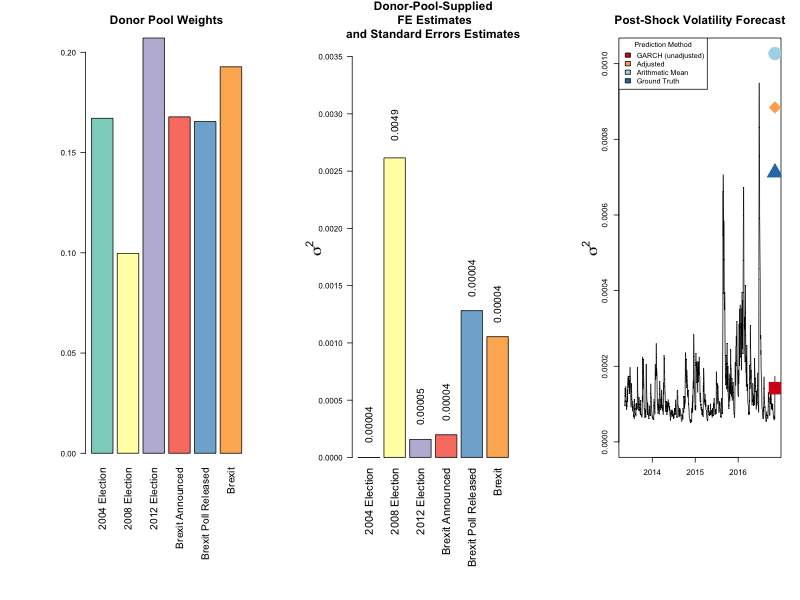
\includegraphics[scale=.6]{real_data_output_plots/TueSep241059512024_IYG_None_None.png}
    \caption{Donor pool weights (left panel), individual shock effects (center panel), and forecasts (right panel).}
    \label{fig:SVF_2016_with_Brexit}
    \end{center}
  \end{figure}


  \begin{table}[ht]
    \centering
    \captionof{table}{Adjusted volatility forecasts for the 2016 US presidential election ranked by QL loss. This table contains all forecasts made by applying simultaneous leave-one-out approaches made to the covariates and the donors forming the donor pool. The forecast from our analysis in the main text is included in yellow. The mean and median of all forecasts is also included in grey.} \label{tab:multiverse_table} 
    \begingroup\fontsize{7pt}{6.5pt}\selectfont
    \begin{tabular}{ccc}
      
      \hline
      QL Loss of the Adjusted Forecast& Omitted Covariate & Omitted Donor \\ 
         \hline
    0.0001 & Log Return of \verb|^|IRX & None \\ 
    \rowcolor{gray} 0.0007 & NA (Average Adjusted Forecast) & NA (Average Adjusted Forecast)\\  
      0.0007 & Log Return of CL=F & 2004-11-02 \\ 
      0.0008 & Log Return of \verb|^|IRX & 2004-11-02 \\ 
      0.0034 & Log Return of \verb|^|TNX & None \\ 
      0.0060 & Log Return of \verb|^|TNX & 2004-11-02 \\ 
      0.0061 & Log Return of \verb|^|VIX & 2016-02-19 \\ 
      0.0077 & Raw\verb|^|VIX & 2004-11-02 \\ 
      0.0079 & None & 2004-11-02 \\ 
      0.0080 & Log Return of CL=F & 2008-11-04 \\ 
      0.0099 & Log Return of \verb|^|VIX & 2004-11-02 \\ 
      \rowcolor{gray}  0.0099 & NA (Median Adjusted Forecast) & NA (Median Adjusted Forecast)\\  
      0.0115 & Log Return of CL=F & 2016-02-19 \\ 
      0.0127 & None & 2016-02-19 \\ 
      0.0137 & Raw\verb|^|VIX & 2016-02-19 \\ 
      0.0151 & Log Return of \verb|^|TNX & 2016-02-19 \\ 
      0.0160 & Log Return of \verb|^|TYX & 2016-02-19 \\ 
      0.0193 & Raw\verb|^|VIX & 2016-06-23 \\ 
      0.0194 & Log Return of \verb|^|VIX & 2016-06-23 \\ 
      0.0216 & Log Return of \verb|^|IRX & 2016-06-23 \\ 
      \rowcolor{yellow} 0.0219 & None & None \\ 
      0.0222 & Log Return of \verb|^|FVX & 2016-02-19 \\ 
      0.0232 & Log Return of \verb|^|VIX & 2008-11-04 \\ 
      0.0237 & Log Return of \verb|^|TNX & 2016-06-23 \\ 
      0.0240 & Log Return of \verb|^|IRX & 2016-02-19 \\ 
      0.0245 & Log Return of \verb|^|TNX & 2008-11-04 \\ 
      0.0251 & None & 2016-06-23 \\ 
      0.0280 & Log Return of CL=F & 2016-06-23 \\ 
      0.0315 & Log Return of \verb|^|FVX & 2008-11-04 \\ 
      0.0322 & None & 2008-11-04 \\ 
      0.0360 & Log Return of \verb|^|TYX & 2008-11-04 \\ 
      0.0393 & Log Return of \verb|^|VIX & 2012-11-06 \\ 
      0.0396 & Raw\verb|^|VIX & 2008-11-04 \\ 
      0.0473 & Log Return of \verb|^|IRX & 2008-11-04 \\ 
      0.0484 & IYG & 2004-11-02 \\ 
      0.0499 & Log Return of \verb|^|FVX & 2016-06-23 \\ 
      0.0542 & Log Return of \verb|^|TYX & 2016-06-23 \\ 
      0.0578 & IYG & 2012-11-06 \\ 
      0.0595 & Log Return of \verb|^|VIX & None \\ 
      0.0596 & Raw\verb|^|VIX & None \\ 
      0.0598 & Log Return of \verb|^|TYX & None \\ 
      0.0598 & IYG & None \\ 
      0.0598 & Log Return of \verb|^|FVX & None \\ 
      0.0604 & Log Return of \verb|^|TYX & 2004-11-02 \\ 
      0.0627 & Log Return of \verb|^|FVX & 2004-11-02 \\ 
      0.0651 & Log Return of CL=F & None \\ 
      0.0692 & Log Return of \verb|^|VIX & 2016-06-13 \\ 
      0.0758 & Log Return of \verb|^|IRX & 2012-11-06 \\ 
      0.0922 & IYG & 2008-11-04 \\ 
      0.0924 & Log Return of \verb|^|TNX & 2012-11-06 \\ 
      0.0990 & None & 2012-11-06 \\ 
      0.1038 & Raw\verb|^|VIX & 2012-11-06 \\ 
      0.1117 & Log Return of \verb|^|IRX & 2016-06-13 \\ 
      0.1147 & Log Return of CL=F & 2012-11-06 \\ 
      0.1241 & Raw\verb|^|VIX & 2016-06-13 \\ 
      0.1356 & IYG & 2016-06-23 \\ 
      0.1359 & Log Return of \verb|^|TYX & 2012-11-06 \\ 
      0.1480 & Log Return of \verb|^|FVX & 2012-11-06 \\ 
      0.1621 & None & 2016-06-13 \\ 
      0.1630 & Log Return of \verb|^|TNX & 2016-06-13 \\ 
      0.1928 & Log Return of CL=F & 2016-06-13 \\ 
      0.2102 & Log Return of \verb|^|FVX & 2016-06-13 \\ 
      0.2435 & Log Return of \verb|^|TYX & 2016-06-13 \\ 
      0.3013 & IYG & 2016-02-19 \\ 
      1.0261 & IYG & 2016-06-13 \\
      \rowcolor{red} 2.3529 & All & All \\ 
       \hline
    \end{tabular}
    \endgroup
    \end{table}\label{multiverse_table}

\section{Discussion}

This present work applies and innovates techniques in similarity-based forecasting and information aggregation in order to provide better GARCH forecasts under news shocks.  It extends \citet{lin2021minimizing} principally by substituting a GARCH model for an AR(1), i.e. by modeling both the mean and volatility of a univariate time series.  An interesting connection insight related to \citet{lin2021minimizing} is that the GARCH model, under weak assumptions, can be represented as an ARMA on the squared residuals $a^{2}_{t}$.  Hence, a shock $\omega^{*}_{i,t}$ to the volatility at time $t$ is an identical shock to $a^{2}_{t}$. However, this use-case becomes less attractive in situations where the sign of the time series under study following the shock is uncertain.  Insofar as this work has made advances that accommodate heteroskedastic time series, the benefits may redound most amply to applications like Value-At-Risk (VaR) and Expected Shortfall, where $\hat\sigma^{2}_{t}$ is an input.

This work as well as \citet{lin2021minimizing} itself can be viewed as a generalization of \cite{phillips1996forecasting} where the rare event probability $\lambda$ is assumed to be 1 and the error associated with the rare event is estimated using external series.  In our setting, if the shock to the time series under study were known and yet so underdescribed, i.e. so lacking in qualitative context, then \cite{phillips1996forecasting} would be recommended.  However, in our setting the rare event is not only rare but also contains specific qualitative features that are best accounted for via data aggregation.

The method under development does not strictly require knowledge of the length of the shocks in the donor pool, but correctly sizing up those shock lengths is helpful to proper estimation of the shocks in the donor pool.  An important question remains: even if the donor pool shock lengths are assumed to be known, how do we advise the operator to forecast the time series under study?  In other words, for how long is the adjustment estimator $\omega^{*}$ valid, applicable, and reliable?  One idea suggested by the paper is obvious: why not aggregate the shock lengths from the donors as well and round that quantity or take the floor or ceiling of any non-integer value?  This is worth pursuing.  However, it may be that estimating the persistence of a volatility shock induced by news is an endeavor deserving of its own study, where aggregation methods might naturally arise as helpful tools.

There is also a broader discussion to be had regarding the degree of model heterogeneity permitted in fitting the donors' series.  

\subsection{Comparison with KNN}

\cite{clements1996intercept} (cited in \cite{guerron2017macroeconomic})  note intercept corrections find their theoretical basis in the occurrence of structural breaks, whereas Nearest-Neighbor methods, being nonparametric, are theoretically more adept at accounting for nonlinearity.  The present work examines news shocks, which are more closely related to structural breaks (though though one could easily imagine more exotic conditional shock distributions, including nonlinearity in the covariates).  Nevertheless, there are deeper observations to be made about KNN.  The method presented here is unlike KNN in that we are not trying to learn a function, first and foremost.  We are trying to estimate a parameter.  Also, KNN encounters the curse of dimensionality.  In contrast, large $p$ is not a problem in Synthetic Control and related methods, since the intermediary object estimated is the vector $\weight$ with $n-1$ degrees of freedom.  For KNN, a high-dimensional space, i.e. large $p$, corresponding to many covariates, is a difficult space in which to work with distances \citep{hastie2009elements}.  In contrast, large $p$ is not a problem in and of itself for Synthetic Control --- in fact, asymptotic results exist for $p$ \citep{abadie2010synthetic}.  

As is pointed out in \citet{hastie2009elements}, KNN regression performs well when $K$ is chosen small enough that one can simply average the points $\{y_{i}\}_{i=1}^{N_{train}}$in the neighborhood around each element in $\{y_{i}\}_{i=1}^{N_{test}}$ to get good predictions.  As we have noted above, the arithmetic mean-based estimator of $\omega^{*}$, denoted $\overline{\omega^{*}}$, corresponds to KNN when $K = n$, the number of donors.  Fundamentally, the idea that $n$ would be small enough and the donors homogeneous enough that one could simply average the $\hat\omega_{i,*}$ is at odds with the assumed variation in the shocks in our modeling setup, and the real data example attests to what can do wrong when that variation is not accounted for.

Additionally, in KNN regression, the hyperparameter K must be learned.  In similarity-based parameter correction, the number of donors is not learned.  A donor pool is curated, and then careful rules of thumb can be applied to determine whether a given donor should be included or excluded.  This brings us to a deeper point about the distinction between similarity-based methods in the style of \citet{lin2021minimizing} and KNN.  In KNN, the exogenous variables are taken as a given and nearness to the object to be predicted depends on the distance function chosen.  In contrast, in \citet{lin2021minimizing}, the determination of nearness begins with a qualitative step, i.e. curating the donor units between which we will calculate distances and from which we will ultimately derive weights.

\subsection{Donor Pool Construction}

Should we gather as many donors as possible and pick them quantitatively?  It would be counter to the method proposed to assemble a vast number of donors, lacking careful scrutiny of the qualitative fit, and let the optimization simply pick the donors, via weighting.  What makes a donor good is not merely its quantitative fit but its qualitative fit as well.  \citet{abadie2022synthetic} make a similar point about large donor pools.  

What matters is that the donors chosen are properly situated in the $p$-dimensional predictor space, so as to allow proper estimation of the weights.  %For more on this question, see the Supplement, where the donors and the volatility profile are treated with a leave-one-out analysis.
That being said there may be subjectivity in selecting donors, and care will be needed to make good selections. In this work we included Brexit and the previous three US presidential elections as donors used for forecasting volatility following the 2016 US presidential election. The resulting adjusted forecast with this donor pool performed very well. In our supplement we show that adjusted forecasts perform well under a variety of donor pool choices and covariate choices.

\subsection{The Nature and Estimation of Volatility Shocks}

Not all of the volatility of an asset return may be related to news \citep{boudoukh2019information}.  This explains our inclusion of an idiosyncratic noise term in the shock specification.  However, this point also gestures in the direction of possible unexplained variation in the shocks.  \citet{chinco2019sparse} find that for predicting 1-minute returns, highly transitory firm-specific news is useful.  The authors conclude that news about fundamentals is predictive.

It would be a pyrrhic victory for our method if the volatility profile indeed underlies real-world shocks but the volatility profile is radically high-dimensional or the signal in the shocks is overwhelmed by the noise term.  Even unbiased predictions can be unhelpful if they are high in variability, and in Section \ref{forecastcomb}, we show how the benefits of forecast combination.  Another possibility is high-frequency data and the use of linear models like HAR \citep{corsi2012har}.  HAR would not only increase the sample size available for discovering the autoregressive structure of a series' realized volatility.  It would also open the door to high-dimensional regression methods, shrinkage estimators, and more.

\subsection{Parameter Stability}

There is an important question about the stability of the GARCH parameters under the presence of a shock, and on parameter instability as it pertains to forecasting, we refer readers to \cite{rossi2013advances, rossi2021forecasting}.  There are at least two reasons that we do not explore parameter instability or methods to adjust for it.  First, the marginal effect of coefficient changes at the shock time would, under the assumptions in this work, be swamped by the random effect.  Second, the estimation of post-shock parameter values would require at least several --- better yet, dozens --- of post-shock data points in the time series under study, whereas this work assumes access to zero post-shock data points.  However, it is possible that similarity-based estimators for the GARCH coefficients could be produced, for example, by adapting the methods of \citet{dendramis2020similarity}.

\section{Supplement}

Here we provide additional useful information about the foregoing results and analyses.  We begin with several sections that re-examine the results of our real data example through a multiverse perspective.  We also explore forecast combination as a tool for real data analysis by evaluating the mean and median of the full set of forecasts generated by dropping one covariate and one donor at a time.  Finally, we provide proofs for the numerous formal results found earlier in this work.

\subsection{Leave-one-out: How we analyzed a multiverse of 63 predictions}

Given the option of redoing our analysis, with eight covariates and six donors, a natural question from a place of skepticism is, how stable are the results --- how contingent are they on a particular specification?  To answer these questions, in Table \ref{tab:multiverse_table} we generate all 63 predictions yielded the decision of leave out any one of the donors (or none) and any one of the covariates (or none).  This analysis includes the prediction presented above in Figure \ref{fig:SVF_2016_with_Brexit}, which can be viewed as the null model, at least in the sense that it provides and baseline for comparison. 
 
     
\subsection{Sensitivity to Covariates Chosen}
Any covariate that appears near to the bottom of Table \ref{tab:multiverse_table} more often is, in a greedy sense, a more important covariate for this prediction task, since by dropping it, a larger loss results.  Similarly, any covariate that appears more often in forecasts below the null are covariates that lead to a worse forecast than the null.  The covariate that thus stands out in positive way is the squared, demeaned log return of IYG, of which we use the three days preceeding the date $T_{i}^{*}$.  This suggests that the behavior of the observable time series itself (and its transformation) may be a useful proxy for risk conditions, a result wholly consistent with the core consistency result for Synthetic Control found in \cite{abadie2010synthetic}.

\subsection{Sensitivity to Donors Chosen}

The most glaring result visible in Table \ref{tab:multiverse_table} regarding donor selection is two-fold: on one hand, omitting the donor that is the Brexit Poll of June 13th, 2016 leads to the worst QL Loss quantities, far worse than having the full set of donors.  It could very well be that the poll released that day attenuates the contribution of Brexit itself, and without accounting for the full variety of Brexit-related events in 2016, a poor prediction results.  Hence, the inclusion of all three Brexit donors is justified.  

On the other hand, the 2004 election appears most often at the top of the table, suggesting that is an unhelpful donor.  This is unsurprising if one considers that the fixed effect estimate for 2004 is nearly zero.  That means that by dropping the 2004 election, other donors must account for the approximately 17\% weight it had in the null model.  The donors that fill that void then have the opportunity to vault the prediction much closer to the ground truth.  This discussion hints at a conjecture one might make: that the removal of an unjustified donor will improve forecast performance in expectation, under certain conditions.  More fundamentally, however, we should ask why it is that 2004 is such a poor donor, beyond the fact that its fixed effect is small.  It could be that the 2004 election delivered such little surprise or is so far distant, temporally, that its inclusion in our donor pool is not fully justified.  The potential lesson to practitioners of the method is that even when there appears to be a default donor pool available, some degree of curation and vetting may be beneficial.

% \subsubsection{Brexit}

% Defining exactly when Brexit occurred is requires some care because of the time zone differences between the UK and the US make difficult the analysis of after-hour shocks on US markets.  Additionally, like many election results, that the ``Leave'' side of the referendum would prevail was not revealed at any discrete time, of course, but became more certain as observation of voting turnout and informal vote tallies across the UK progressed \citep{BBC_News_2016}.  This is in spite of UK news outlets adhering to various rules and guidelines regarding reportage of polling results \citep{Bailey_2024}.  These facts pose a challenge for any method that uses daily data.  In our analysis we defined Brexit
% %Of prime concern is whether we should consider $T^{*}$ for Brexit 
% to have occurred after market hours on June 22nd, 2016, which implies that $T_{Brexit}^{*}+1$ is June 23rd, 2016, and hence the reaction of IYG to Brexit can be estimated and extracted from late-day trading on that date. Alternatively, one could have defined Brexit as occurring on June 23rd, 2016, implying that $T_{Brexit}^{*}+1$ is June 23rd, 2016. Such a choice may ignore the steady percolation of information and uncertainty that attend election days. A leave-one-out analysis with Brexit defined as occurring on June 23rd, 2016 is presented in Table~\ref{tab:prediction_table_with Brexit as June 23rd, 2016}. A breakdown of donor weights, fixed effect estimates, and adjusted forecasts with Brexit defined as occurring on June 23rd, 2016 is included in Figure~\ref{fig:SVF_2016_with_Brexit_06-23}. 

%, or alternatively, consider the shock to have occurred after hours on June 22nd, 2016, which implies that $T^{*}+1$ is June 23rd, 2016, and hence the reaction of IYG to Brexit can be estimated and extracted from late-day trading on that date. 


%In the pre-quantitative analysis of donors, there was only one competitor to the setup that was ultimately selected and presented in Section \ref{Real Data Example}, and that competitor donor pool used Brexit.  The inclusion of Brexit is based on the fundamental belief that the conditional shock distribution governing IYG's volatility shocks may be shared among US elections and some political events elsewhere, like the Brexit referendum of July 23rd, 2016.  That referendum shared some important qualities with the 2016 US elections, which we have discussed above.

%We now turn, however, to why the inclusion of Brexit failed to perform nearly as well our primary specification.  First, note time zone differences between the UK and the US make difficult the analysis of after-hour shocks on US markets.  Additionally, like many election results, that the ``Leave'' side of the referendum would prevail was not revealed at any discrete time, of course, but became more certain as observation of voting turnout and informal vote tallies across the UK progressed \citep{BBC_News_2016}.  This is in spite of UK news outlets adhering to various rules and guidelines regarding reportage of polling results \citep{Bailey_2024}.  These facts pose a challenge for any method that uses daily data.  Of prime concern is whether we should consider $T^{*}$ for Brexit to have occurred after market hours on June 23rd, 2016, Eastern Standard Time, which ignores the steady percolation of information and uncertainty that attend election days, or alternatively, consider the shock to have occurred after hours on June 22nd, 2016, which implies that $T^{*}+1$ is June 23rd, 2016, and hence the reaction of IYG to Brexit can be estimated and extracted from late-day trading on that date.  Given this dilemma, we opt for dropping Brexit from our predictive model completely.

%\begin{figure}[H]
%\begin{center}
%  \textbf{Real Data Example: 2016 Election}\par\medskip
%  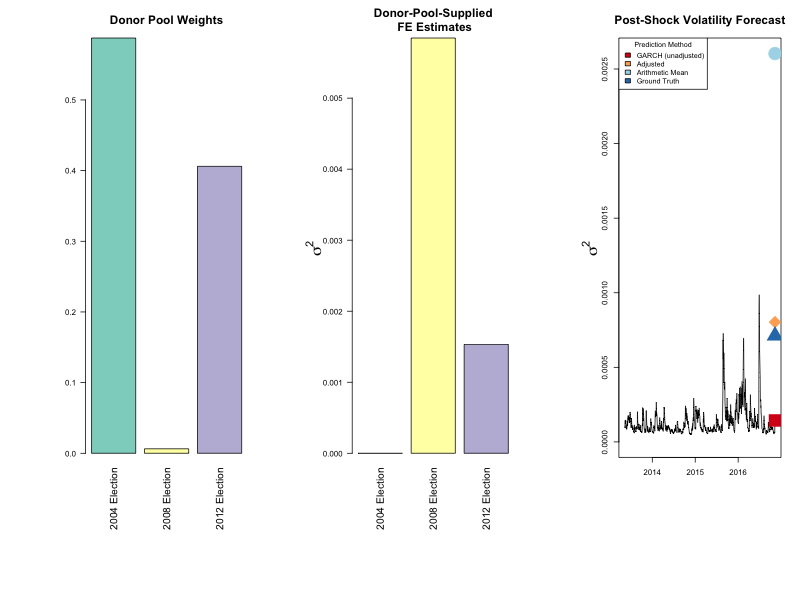
\includegraphics[scale=.5]{real_data_output_plots/FriMay311830522024_IYG_None_2016-06-22.png}
%  \caption{The volatility induced by the 2016 US election}
%  \label{fig:SVF_2016}
%  \end{center}
%\end{figure}

\subsection{Can we combine forecasts to outperform the individual forecasts?}\label{forecastcomb}

We consider a very simple forecast combination procedure -- in fact, we consider two: the average forecast and the median forecast.  While forecast combination can be justified in any number of ways, here we invoke forecast combination as a way to robustify forecasts against misspecification.  We combine in two simply ways, using the mean of all 63 forecasts and the median of all 63 forecasts.  The forecast losses are all specifications -- including the average and median forecasts -- are presented in Table \ref{tab:multiverse_table}.

%\begin{figure}[H]
%  \begin{center}
%    \textbf{Real Data Example: 2016 Election with Brexit as June 22nd, 2016}\par\medskip
%    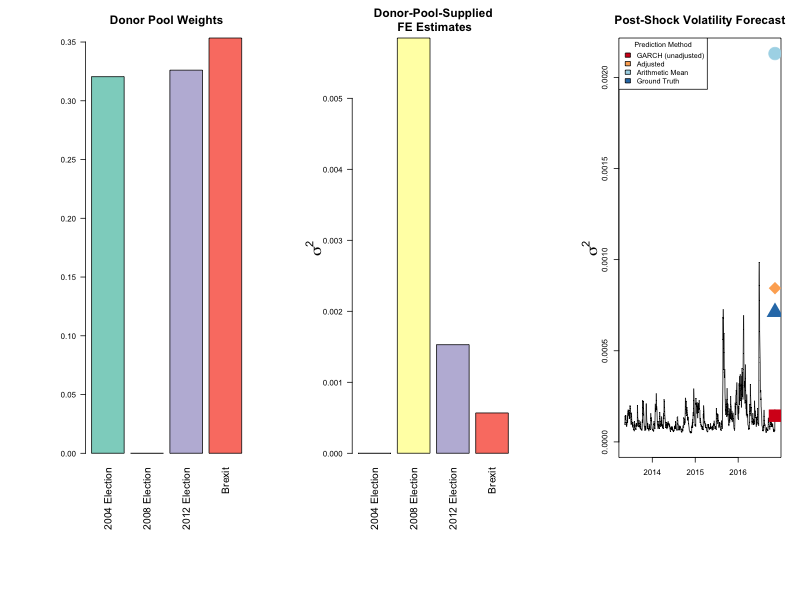
\includegraphics[scale=.6]{real_data_output_plots/FriMay311830182024_IYG_None_None.png}
%    \caption{When Brexit is taken to be June 22nd, 2016, it is shares equal weight with the 2004 and 2008 elections, while its modest fixed effect estimate is the smallest of the three nonzero estimates.}
 %   \label{fig:SVF_2016_with_Brexit}
 %   \end{center}
 % \end{figure}


  

  % \begin{figure}[H]
  %   \begin{center}
  %     \textbf{Adjusted volatility forecast following the 2016 US presidential election with Brexit as June 23rd, 2016}\par\medskip
  %     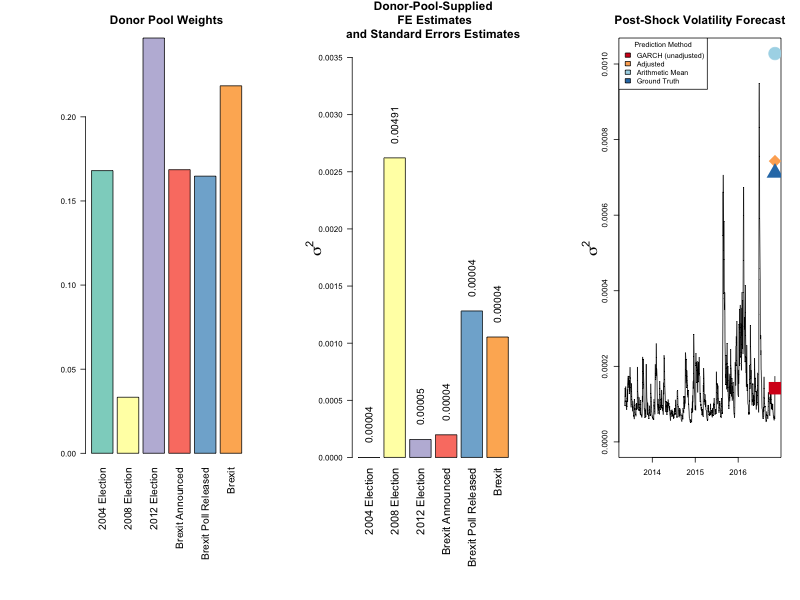
\includegraphics[scale=.6]{real_data_output_plots/WedSep182237432024_IYG_None_None.png}
  %     \caption{When Brexit is taken to be June 23rd, 2016, its own weight is unchanged but others' weights are.  The large fixed effect estimate of Brexit contributes to an overprediction.}
  %     \label{fig:SVF_2016_with_Brexit_06-23}
  %     \end{center}
  %   \end{figure}

    

    % \begin{figure}[H]
    %   \begin{center}
    %     \textbf{Adjusted volatility forecast following the 2016 US presidential election with Brexit as June 23rd and June 24th, 2016}\par\medskip
    %     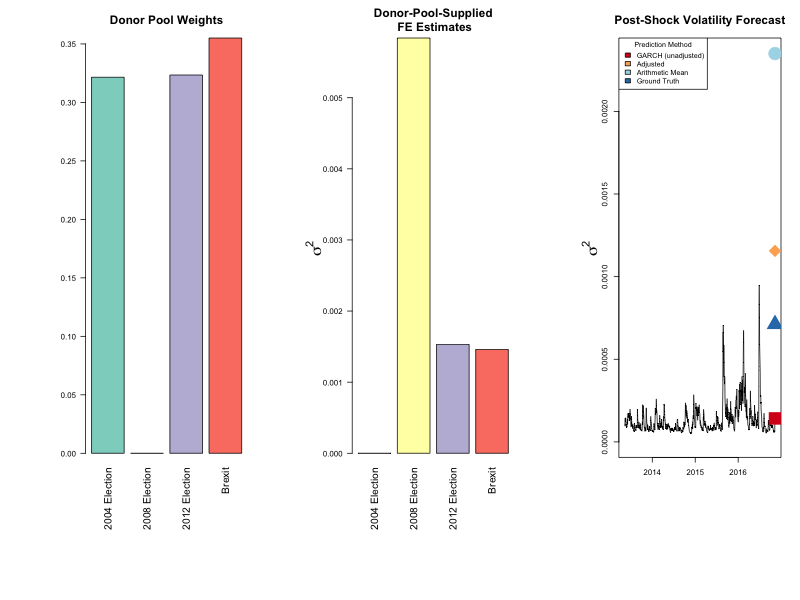
\includegraphics[scale=.6]{real_data_output_plots/WedSep041316522024_IYG_None_None.png}
    %     \caption{When the Brexit shock is taken to be $T_{Brexit}^{*}$ = June 22nd, 2016 and begin with $T_{Brexit}^{*}+1$ June 23rd, 2016, and last through June 24th, 2016, its own weight is still unchanged.  The fixed effect estimate of the shock is large, but not as large when the shock is taken to be June 23rd, 2016.}
    %     \label{fig:SVF_2016_with_Brexit_06-23_through_6-24}
    %     \end{center}
    %   \end{figure}

\subsection{Formal Results}

\begin{proof-of-proposition}[\ref{decay_prop}]
  We claim
  \begin{align}
  \mathbb{E}[ \sigma^{2}_{i,T_{i}^{*}+r+1} |\mathcal{F}_{T_{i}^{*}+r}] & = \mathbb{E}[\omega_{i} + \alpha a_{T_{i}^{*}+r}^{2} + \beta\sigma^{2}_{i,T_{i}^{*}+r} |\mathcal{F}_{T_{i}^{*}+r}] \label{eq1}\\
  & = \omega_{i} + \mathbb{E}[\alpha(\sigma_{i,T^{*}+r}\epsilon_{T_{i}^{*}+r})^{2} |\mathcal{F}_{T_{i}^{*}+r}] + \beta\sigma^{2}_{i,T_{i}^{*}+r} \label{eq2}\\
  & = \omega_{i} + \alpha\sigma_{i,T_{i}^{*}+r}^{2} + \beta\sigma^{2}_{i,T_{i}^{*}+r} \label{eq3}\\
  & = \omega_{i} + (\alpha + \beta) \sigma^{2}_{i,T_{i}^{*}+r}\label{eq4} \text{ .}
  \end{align}
  The volatility equation of a GARCH(1,1) dictates that for any $r$, the one-step-ahead volatility is given by the expression inside the expectation in \eqref{eq1}.  By the mean-model assumption of a GARCH(1,1), we have $a_{i,t} = \sigma_{i,t}\epsilon_{i,t}$, and hence by substituting $\sigma_{i,t}\epsilon_{i,t}$ for $a_{i,t}$, we arrive at equation \eqref{eq2} above.  Using the unit-variance assumption on $\epsilon_{T_{i}^{*}+r}$, we can compute explicitly the expectation, yielding (\ref{eq3}).  Finally, by rearranging terms, we arrive at equation \eqref{eq4}.
  \end{proof-of-proposition}

  \begin{proof-of-lemma}[\ref{lemma_ref}]
    Since the shock is assumed to arrive uniformly at random for each $i$, $1 \leq i \leq n + 1$, and last for a discrete number of indices, the sequence $\{\omega_{i,t}^{*}\}_{t=0,...,T_i}$ is governed by a distribution $F_{\{\omega_{i,t}^{*}\}_{t=0,...,T_i}}$ that is invariant to shifts in time and thus satisfies strong stationarity.
    \end{proof-of-lemma}
    
    \begin{proof-of-proposition}[\ref{adjustment}]
    The result follows from the consistency proof of the QMLE in GARCH-X models, as established by \citet{han2014asymptotic}. 
    \end{proof-of-proposition}

    \begin{proof-of-proposition}[\ref{sigma_consistency}]
      Without loss of generality, we prove the case for $r = 1$.  The general case follows from iterative one-step-ahead forecasts.  Recall the conditional expectation of the variance for the GARCH-X($m$,$s$) model:
      \begin{align*}
      \E[\sigma^{2}_{i,t+1}|\mathcal{F}_{t}] = \omega_{i} +  \sum^{m_{i}}_{k=1}\alpha_{i,k}a^{2}_{i,t+1-k} + \sum_{j=1}^{s_{i}}\beta_{i,j}\sigma_{i,t+1-j}^{2} + \gamma_{i}^{T} \x_{i,t+1} + \omega^{*}_{i,*} \text{ .}
      \end{align*}
      By replacing parameters with their estimates, we arrive at the prediction 
      \begin{align*}
      \hat\sigma^{2}_{i,t+1}|\mathcal{F}_{t} = \hat\omega_{i} + \sum^{m_{i}}_{k=1}\hat\alpha_{i,k}a^{2}_{i,t+1-k} + \sum_{j=1}^{s_{i}}\hat\beta_{i,j}\hat\sigma_{i,t+1-j}^{2} + \hat\gamma_{i}^{T} \x_{i,t+1} + \hat\omega^{*}_{i,*}\text { ,}
      \end{align*}
      which converges in probability to 
      \begin{align*}
        \sigma^{2}_{i,t+1}|\mathcal{F}_{t} = \omega_{i} + \sum^{m_{i}}_{k=1}\alpha_{i,k}a^{2}_{i,t+1-k} + \sum_{j=1}^{s_{i}}\beta_{i,j}\sigma_{i,t+1-j}^{2} + \gamma_{i}^{T} \x_{i,t+1} + \omega^{*}_{i,*}
        \end{align*}
      
      as $t\rightarrow\infty$ by a simple application of Slutsky's Theorem.
      \end{proof-of-proposition}

  \begin{proof-of-proposition}[\ref{asymptotic_consistency}]
    First, note that the function $g:(-\infty,\omega_{i}^{*})\rightarrow \mathbb{R}$ given by $g(x) = \frac{x}{\sigma^{2}_{t+1}-x} + \log{\frac{\sigma_{t+1}^{2}-x}{\sigma_{t+1}^{2}} }$ is nonnegative, convex, obtains a minimum at $x = 0$, and being continuous, preserves consistency. The conclusion follows from facts that the model is correctly specified and the consistency of $\hat\sigma^{2}_{t+1, adjusted}$ is guaranteed by Proposition ($\ref{sigma_consistency}$). 
  \end{proof-of-proposition}
  
\clearpage

\bibliography{synthVolForecast}

\end{document}